\documentclass[a4paper, 12pt]{article}
\usepackage[left=2.5cm, right=2.5cm, top=3cm, bottom=3cm]{geometry}
\usepackage[spanish]{babel}
\usepackage{amsmath}
\usepackage{graphicx}
\usepackage{color}
\usepackage[utf8]{inputenc}
\usepackage[T1]{fontenc}
\usepackage{listings}
\usepackage{booktabs}
\usepackage{longtable}
\usepackage{array}
\usepackage[table]{xcolor}
\newcolumntype{d}{D{.}{.}{-1}}
\definecolor{lightgray}{rgb}{0.95,0.95,0.95}

\usepackage{tikz}
\usetikzlibrary{shapes,arrows,positioning}

\definecolor{colorgreen}{rgb}{0,0.6,0}
\definecolor{colorgray}{rgb}{0.5,0.5,0.5}
\definecolor{colorpurple}{rgb}{0.58,0,0.82}
\definecolor{colorback}{RGB}{255,255,204}
\definecolor{colorbackground}{RGB}{200,200,221}
%Definiendo el estilo de las porciones de codigo
\lstset{
 backgroundcolor=\color{colorbackground},
commentstyle=\color{colorgreen},
keywordstyle=\color{colorpurple},
numberstyle=\tiny\color{colorgray},
stringstyle=\color{colorgreen},
basicstyle=\ttfamily\footnotesize,
breakatwhitespace=false,
breaklines=true,
captionpos=b,
keepspaces=true,
numbers=left,
showspaces=false,
showstringspaces=false,
showtabs=false,
tabsize=2,
frame=single,
framesep=2pt,
rulecolor=\color{black},
framerule=1pt
}



\begin{document}
\graphicspath{{./}}

\begin{center}
\text{\huge \textbf{Informe del Proyecto Final} }\\
\vspace {0.5cm}
\text{\huge \textbf{de}}\\
\vspace {0.5cm}
\text{\huge \textbf{Estadística}}\\
\vspace {5cm}
\text{\huge Richard Alejandro Matos Arderí}\\
\text{\huge Mauricio Sunde Jiménez}\\
\vspace {1cm}
\vspace {2cm}
\text{\Large Grupo 311, Ciencia de la Computación.}\\
\vspace {0.5cm}
\text{\Large Facultad de Matemática y Computación}\\
\text{\Large Universidad de La Habana.}\\
\vspace {0.5cm}
\begin{figure}[h]
    \centering
    
\includegraphics[width=0.2\textwidth, height=0.2\textheight]{MATCOM.jpg}
\end{figure}
\vspace {0.5cm}
\text{2024}\\


\end{center}

\newpage
\tableofcontents
\newpage

\section{Introducción}

 Este proyecto de análisis estadístico, realizado como parte del plan de estudios de Ciencia de la Computación, se centra en el conjunto de datos \textbf{Breast Cancer Wisconsin (Diagnostics)}. Este dataset, ampliamente utilizado en la investigación de aprendizaje automático y análisis de datos biomédicos, contiene información crucial para la clasificación de tumores mamarios como benignos o malignos. Nuestro objetivo es ir más allá de una simple clasificación y profundizar en un análisis estadístico exhaustivo, explorando las características de los datos y sus relaciones intrínsecas.\\

En una primera etapa, emplearemos técnicas de estadística descriptiva para obtener una comprensión inicial del dataset. Esto incluirá el cálculo de medidas de tendencia central (media, mediana, moda) y medidas de dispersión (desviación estándar, varianza, rango intercuartílico) para cada variable, proporcionando una visión general de la distribución de los datos. Además, analizaremos la curtosis para determinar la forma de las distribuciones y la presencia de valores atípicos.\\

Posteriormente, nos adentraremos en el ámbito de la estadística inferencial. Comenzaremos con la estimación puntual y por intervalos de confianza de parámetros clave, como la media y la proporción, para inferir características de la población a partir de la muestra disponible. Realizaremos pruebas de normalidad (Shapiro-Wilk, Kolmogorov-Smirnov) para determinar si las distribuciones de las variables se ajustan a una distribución normal, un requisito para muchas pruebas paramétricas. Además, llevaremos a cabo pruebas de hipótesis sobre los parámetros de la población, examinando si existen diferencias significativas entre los grupos de tumores benignos y malignos.\\

Un aspecto fundamental de este proyecto será el análisis de las relaciones entre variables. Emplearemos técnicas de análisis de correlación (Pearson, Spearman) para identificar la fuerza y dirección de la asociación entre las características del tumor. También realizaremos pruebas de independencia de variables (chi-cuadrado) para evaluar si existe una relación estadísticamente significativa entre variables categóricas. Finalmente, exploraremos pruebas de homogeneidad para comparar la distribución de variables entre diferentes grupos, contribuyendo a una comprensión más profunda de las diferencias entre tumores benignos y malignos.\\

En resumen, este proyecto pretende ofrecer un análisis estadístico completo y riguroso del dataset \textbf{Breast Cancer Wisconsin (Diagnostics)}, utilizando una variedad de técnicas descriptivas e inferenciales para extraer información relevante y contribuir a una mejor comprensión de las características y relaciones entre los atributos de los tumores mamarios. Los resultados obtenidos permitirán una mejor comprensión de los datos y podrán servir como base para futuros análisis y modelos predictivos.\\

\newpage

\section{Análisis Descriptivo de los datos}

A continuación se muestra un cuadro con todas las variables presentes en el dataset, de conjunto con su clasificación estadística y su escala de medición.
\begin{center}
	

        \begin{tabular}{|p{3.5cm}|p{5.5cm}|p{3cm}|p{2.5cm}|}
            \hline
            \textbf{Variable} & \textbf{Descripción} & \textbf{Clasificación Estadística} & \textbf{Escala de Medición} \\
            \hline
            ID & Identificador único del paciente & Cualitativa & Nominal \\
            
            \textcolor{red}{diagnosis} & Diagnóstico del tumor (1 = maligno, 0 = benigno) & Cualitativa & Nominal \\
            
            \textcolor{red}{radius\_mean} & Radio medio de las células del tumor en $\mu$m & Continua & Razón \\
            
            \textcolor{red}{texture\_mean} & Textura media de las células del tumor & Continua & Razón \\
            
            \textcolor{red}{perimeter\_mean} & Perímetro medio de las células del tumor en $\mu$m & Continua & Razón \\
            
            \textcolor{red}{area\_mean} & Área media de las células del tumor en $\mu$m² & Continua & Razón \\
            
            \textcolor{red}{smoothness\_mean} & Suavidad media de las células del tumor & Continua & Razón \\
            
            \textcolor{red}{compactness\_mean} & Compacidad media de las células del tumor & Continua & Razón \\
            
            concavity\_mean & Concavidad media de las células del tumor & Continua & Razón \\
            
            concave points\_mean & Puntos cóncavos medios de las células del tumor & Continua & Razón \\
            
            \textcolor{red}{symmetry\_mean} & Simetría media de las células del tumor & Continua & Razón \\
            
            fractal dimension\_mean & Dimensión fractal media de las células del tumor & Continua & Razón \\
            
            radius\_se & Desviación estándar del radio de las células del tumor & Continua & Razón \\
            
            texture\_se & Desviación estándar de la textura de las células del tumor & Continua & Razón \\
            
            perimeter\_se & Desviación estándar del perímetro de las células del tumor & Continua & Razón \\
            
            area\_se & Desviación estándar del área de las células del tumor & Continua & Razón \\
            
            smoothness\_se & Desviación estándar de la suavidad de las células del tumor & Continua & Razón \\
            
            compactness\_se & Desviación estándar de la compacidad de las células del tumor & Continua & Razón \\
            \hline
            
        \end{tabular}
        
        \begin{tabular}{|p{3.5cm}|p{5.5cm}|p{3cm}|p{2.5cm}|}
        \hline
            
            concavity\_se & Desviación estándar de la concavidad de las células del tumor & Continua & Razón \\
            
            concave points\_se & Desviación estándar de los puntos cóncavos de las células del tumor & Continua & Razón \\
            
        
            
            symmetry\_se & Desviación estándar de la simetría de las células del tumor & Continua & Razón \\
            
            fractal dimension\_se & Desviación estándar de la dimensión fractal de las células del tumor & Continua & Razón \\
            
            
            \textcolor{red}{radius\_worst} & Radio máximo de las células del tumor en $\mu$m & Continua & Razón \\
            
            \textcolor{red}{texture\_worst} & Textura máxima de las células del tumor & Continua & Razón \\
     
            
            \textcolor{red}{perimeter\_worst} & Perímetro máximo de las células del tumor en $\mu$m & Continua & Razón \\
            
            \textcolor{red}{area\_worst} & Área máxima de las células del tumor en $\mu$m² & Continua & Razón \\
            
            \textcolor{red}{smoothness\_worst} & Suavidad máxima de las células del tumor & Continua & Razón \\
            
            \textcolor{red}{compactness\_worst} & Compacidad máxima de las células del tumor & Continua & Razón \\
            
            concavity\_worst & Concavidad máxima de las células del tumor & Continua & Razón \\
            
            concave points\_worst & Puntos cóncavos máximos de las células del tumor & Continua & Razón \\
            
            \textcolor{red}{symmetry\_worst} & Simetría máxima de las células del tumor & Continua & Razón \\
            
            fractal dimension\_worst & Dimensión fractal máxima de las células del tumor & Continua & Razón \\
            \hline
        \end{tabular}
       
\end{center}


 
Se brindará especial atención a las variables en rojo para el análisis. A continuación se expone una caracterización más detallada de las mismas.


\subsection*{\underline{diagnosis}}

 \begin{itemize}
	\item \textit{Descripción:} Variable categórica que indica si el tumor es maligno o benigno.
	\item \textit{Valores posibles:}
	$1$ (Maligno), $0$ (Benigno).
	\item \textit{Medición:} Determinado a partir del análisis histopatológico.
\end{itemize}

	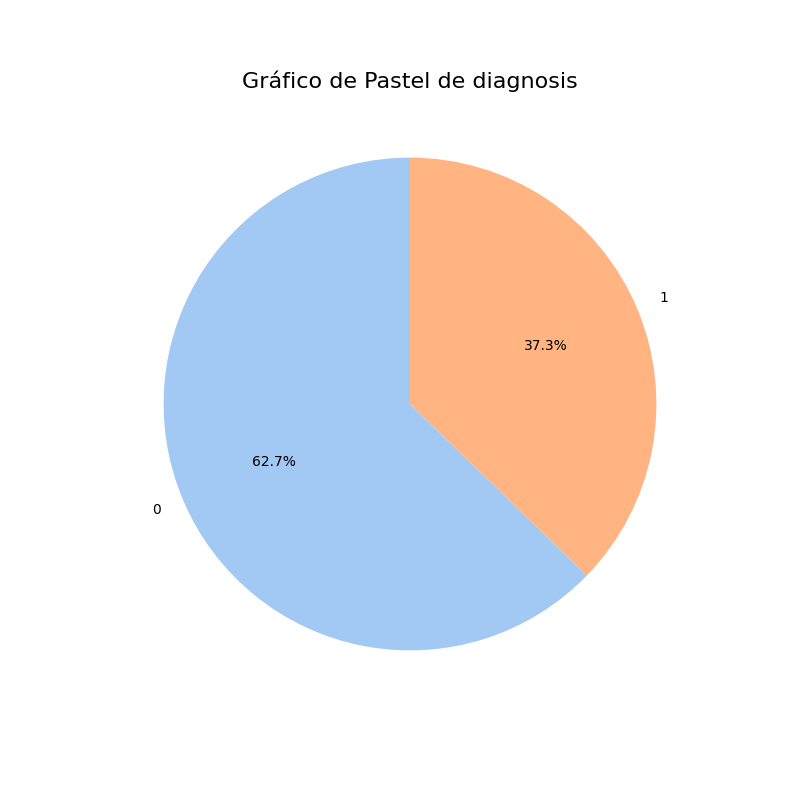
\includegraphics[width=\textwidth]{../Plots/plots_stats/diagnosis/grafico_pastel_diagnosis.png}

	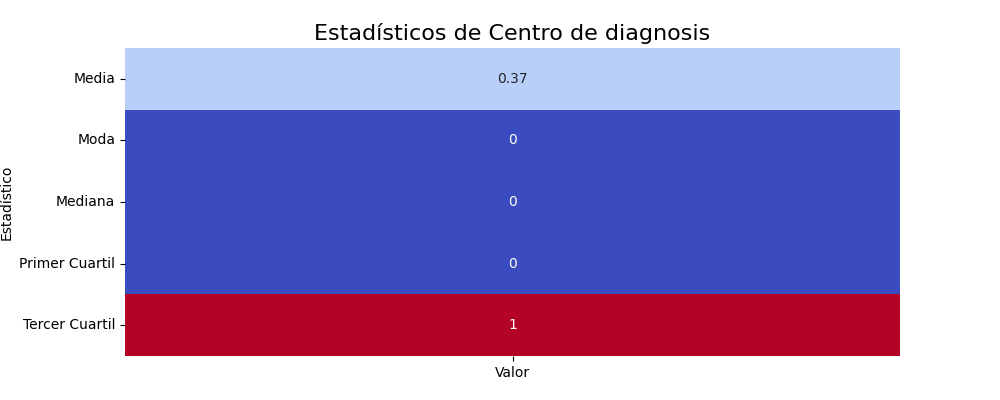
\includegraphics[width=\textwidth]{../Plots/plots_stats/diagnosis/estadisticas_centro_diagnosis.png}

	\includegraphics[width=\textwidth]{../Plots/plots_stats/diagnosis/estadisticos_dispersión_diagnosis.png}

	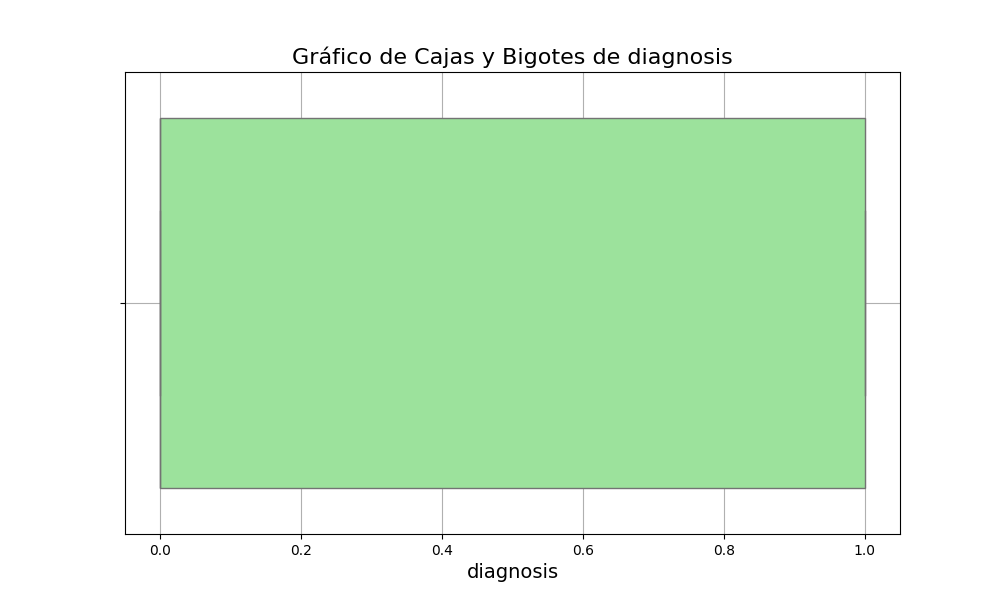
\includegraphics[width=\textwidth]{../Plots/plots_stats/diagnosis/boxplot_diagnosis.png}

	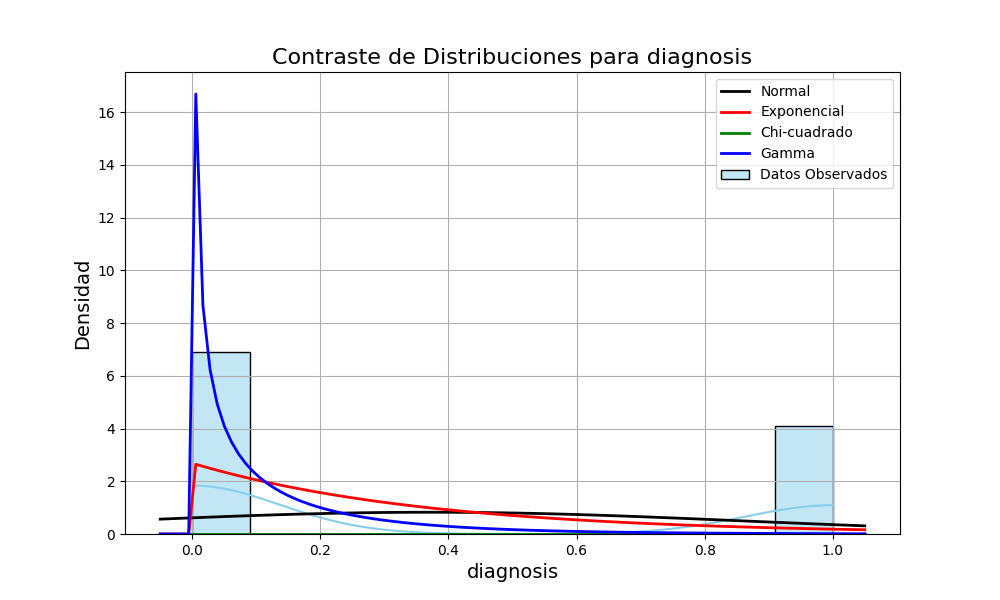
\includegraphics[width=\textwidth]{../Plots/plots_stats/diagnosis/distribuciones_conocidas_diagnosis.png}


\subsection*{\underline{radius\_mean}}

 \begin{itemize}
	\item \textit{Descripción:} Promedio del radio de las células tumorales. La variable es una medida porcentual de una cantidad finita (y contable por tanto), es por esto que aunque encontramos valores racionales la variable se clasifica como cuantitativa discreta. La escala es de razones o proporciones puesto que el cero nos indica ausencia del atributo
	\item \textit{Medición:} Distancia promedio desde el centro hasta el borde.
	\item \textit{Unidades:} Micrómetros ($\mu$m).
	\item \textit{Interpretación:} Valores más altos indican células más grandes, lo cual puede asociarse con malignidad.El \textit{radius\_mean} es una medida importante en la caracterización de los tumores mamarios. Un radio medio mayor puede indicar una mayor probabilidad de malignidad, ya que las células tumorales malignas tienden a ser más grandes. Los gráficos proporcionan una visión detallada de la distribución de esta variable, mostrando su histograma, estadísticas descriptivas, dispersión y comparación con distribuciones conocidas. Además, se observa la relación entre el \textit{radius\_mean} y el diagnóstico, lo que ayuda a entender mejor su impacto en la clasificación de los tumores
\end{itemize}

	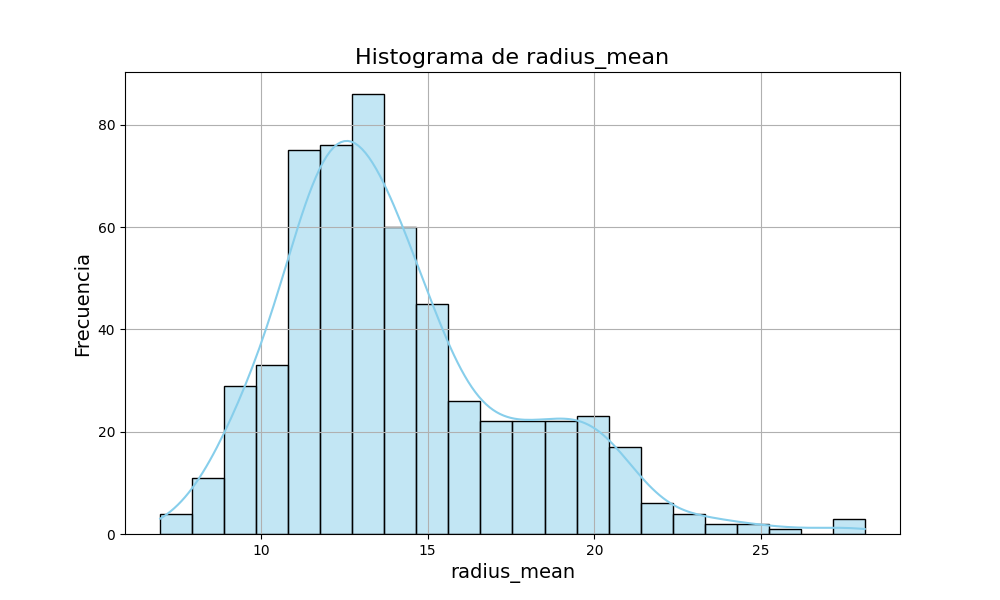
\includegraphics[width=\textwidth]{../Plots/plots_stats/radius_mean/histograma_radius_mean.png}

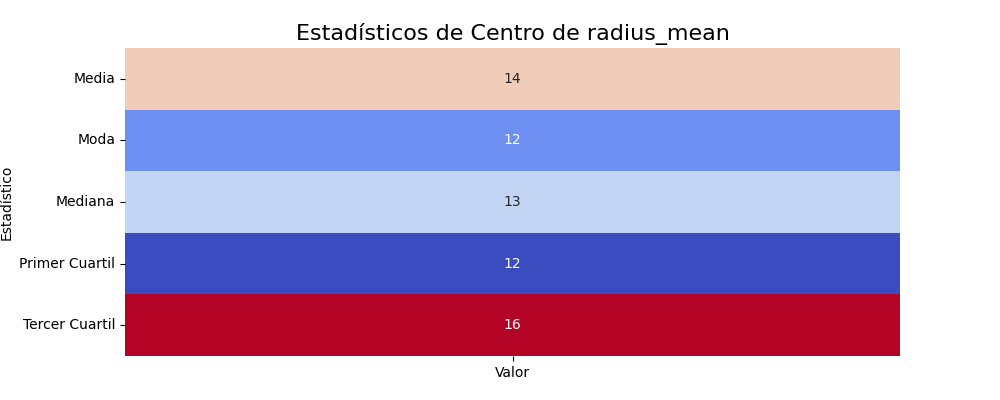
\includegraphics[width=\textwidth]{../Plots/plots_stats/radius_mean/estadisticas_centro_radius_mean.png}

\includegraphics[width=\textwidth]{../Plots/plots_stats/radius_mean/estadisticos_dispersión_radius_mean.png}

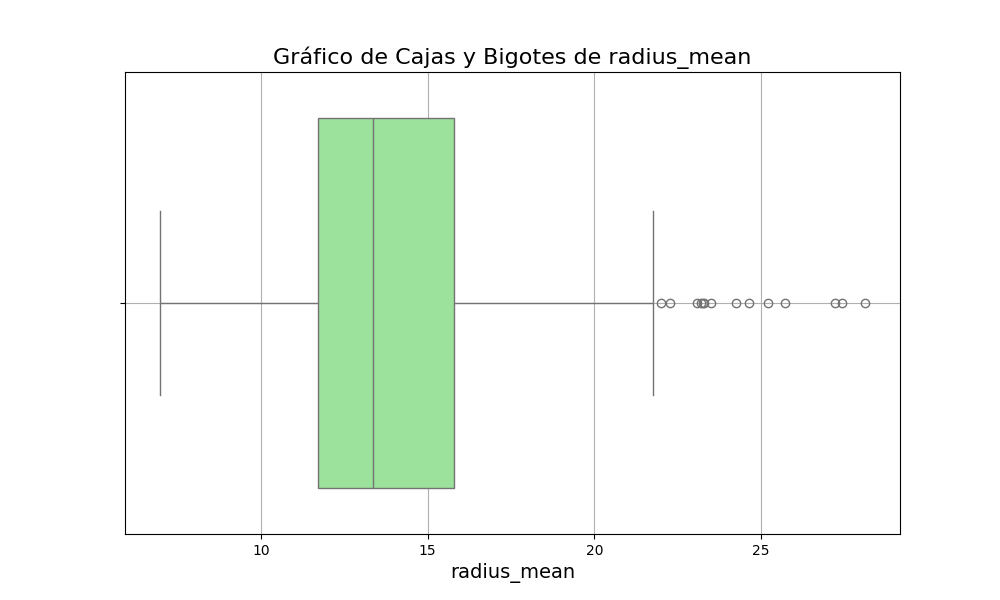
\includegraphics[width=\textwidth]{../Plots/plots_stats/radius_mean/boxplot_radius_mean.png}

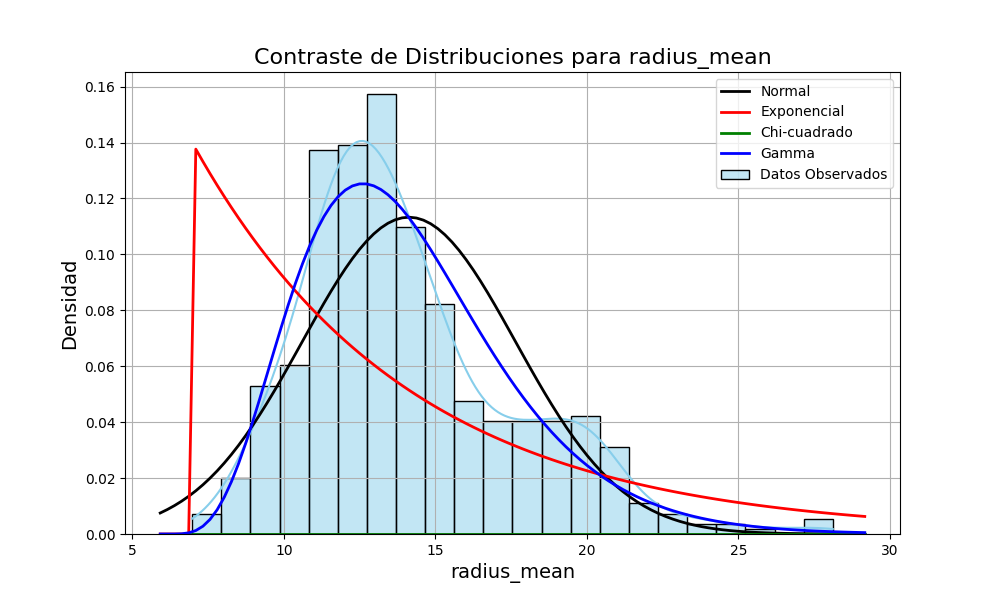
\includegraphics[width=\textwidth]{../Plots/plots_stats/radius_mean/distribuciones_conocidas_radius_mean.png}

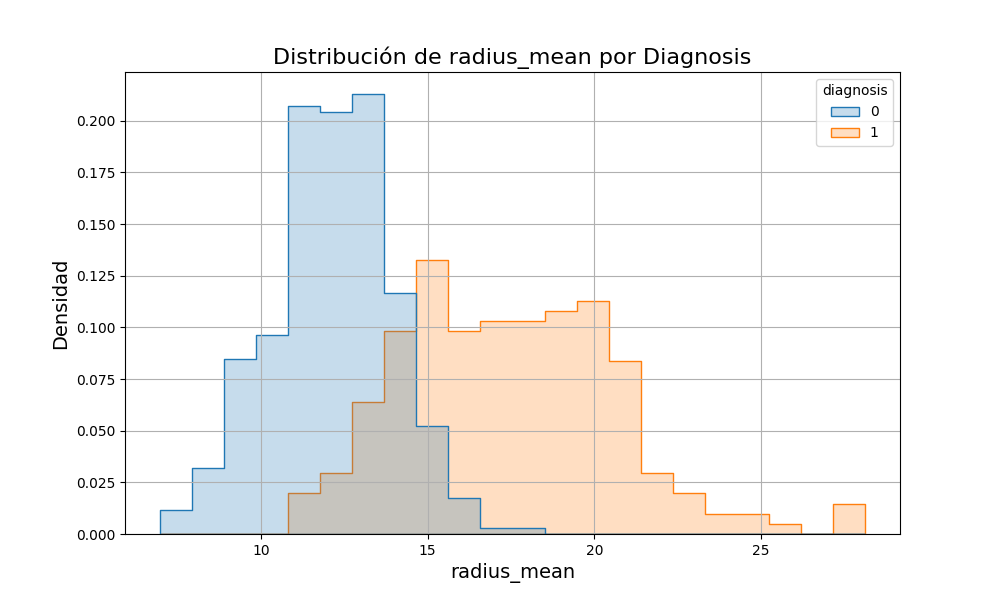
\includegraphics[width=\textwidth]{../Plots/plots_diagnosis/distribucion_radius_mean_por_diagnosis.png}


\subsection*{\underline{texture\_mean}}


    \begin{itemize}
	\item \textit{Descripción:}La textura se relaciona con la variabilidad en la intensidad de los píxeles y puede reflejar características estructurales del tejido.
	\item \textit{Medición:} Promedio de los valores de intensidad.
	\item \textit{Unidades:} Sin unidades (valor adimensional).
	\item \textit{Interpretación:} Valores más altos indican mayor heterogeneidad, lo que sugiere malignidad.
\end{itemize}

	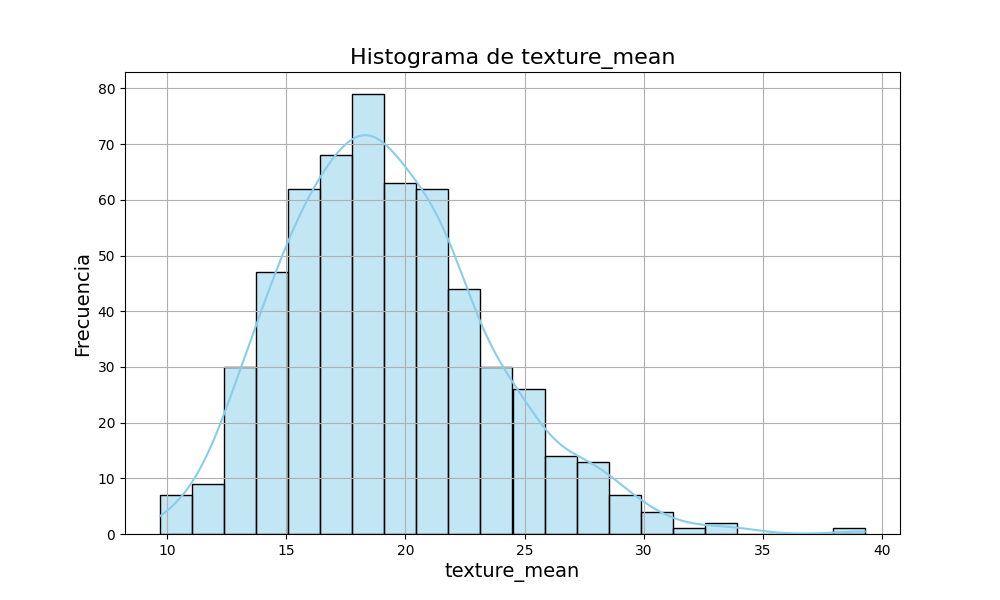
\includegraphics[width=\textwidth]{../Plots/plots_stats/texture_mean/histograma_texture_mean.png}
\begin{itemize}
\item Esta grafica permite visualizar la distribución de la variable.
La distribución es simétrica, por lo que indica que la mayoría de los valores están cercanos a la media.
El análisis del histograma indica que la distribución de la variable texture mean tiene un sesgo positivo (hacia la derecha). Esto significa que la mayoría de los valores están concentrados en la parte baja, mientras que hay una cola extendida hacia valores más altos.
Este tipo de distribución sugiere que hay algunos casos con valores significativamente altos de texture mean, lo que podría indicar la presencia de tejidos con mayor variabilidad en la textura en ciertos casos.
\end{itemize}

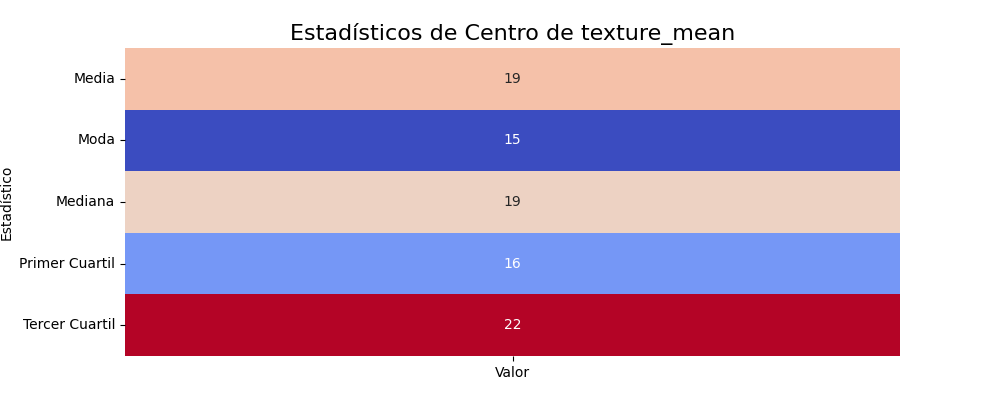
\includegraphics[width=\textwidth]{../Plots/plots_stats/texture_mean/estadisticas_centro_texture_mean.png}

\includegraphics[width=\textwidth]{../Plots/plots_stats/texture_mean/estadisticos_dispersión_texture_mean.png}

Estadísticos de dispersión

\begin{itemize}
\item Incluyen medidas como la desviación estándar y el rango intercuartílico.
\item La alta dispersión indica variabilidad en la textura de las imágenes, lo que podría estar asociado con diferentes tipos de tejidos o estados patológicos.
\end{itemize}

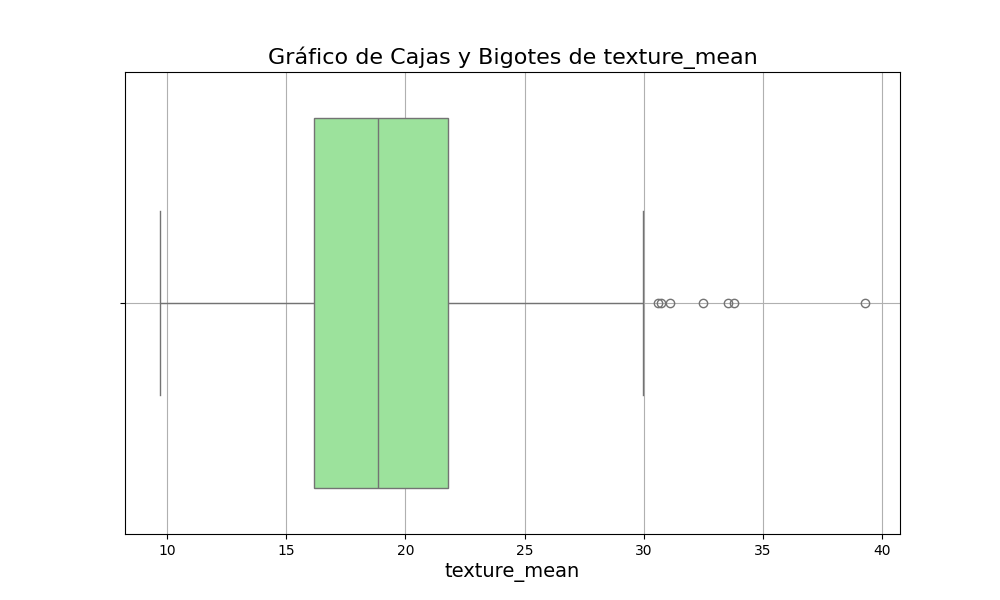
\includegraphics[width=\textwidth]{../Plots/plots_stats/texture_mean/boxplot_texture_mean.png}

Boxplot

\begin{itemize}
\item Muestra la dispersión y posibles outliers (valores atípicos).
\end{itemize}

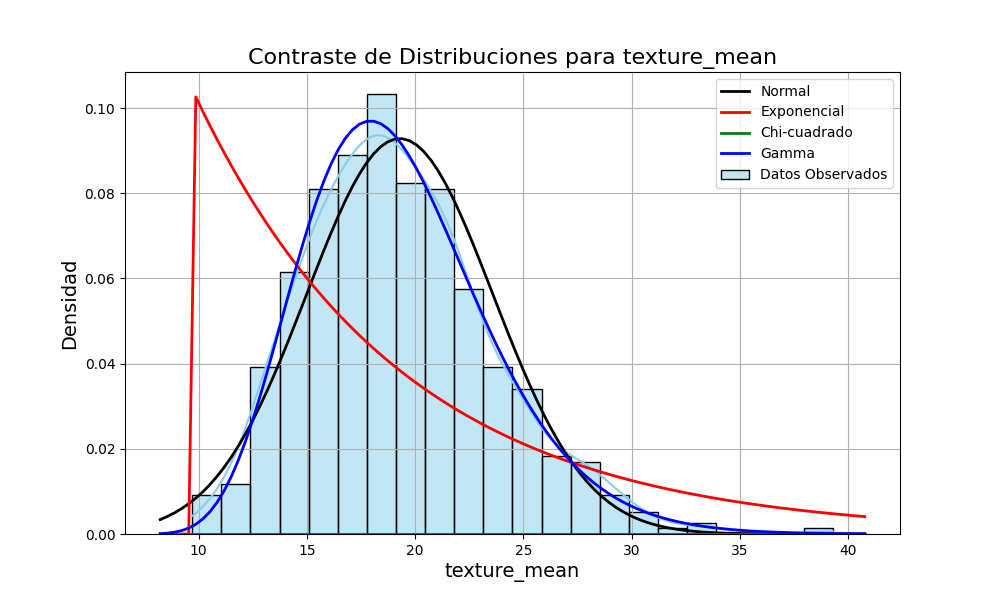
\includegraphics[width=\textwidth]{../Plots/plots_stats/texture_mean/distribuciones_conocidas_texture_mean.png}

Comparación con distribuciones conocidas

\begin{itemize}
\item Permite determinar si la variable sigue una distribución normal o alguna otra (como gamma o log-normal).
\item Si sigue una normal, se pueden aplicar pruebas estadísticas clásicas; si no, pueden requerirse transformaciones o métodos no paramétricos.
\end{itemize}

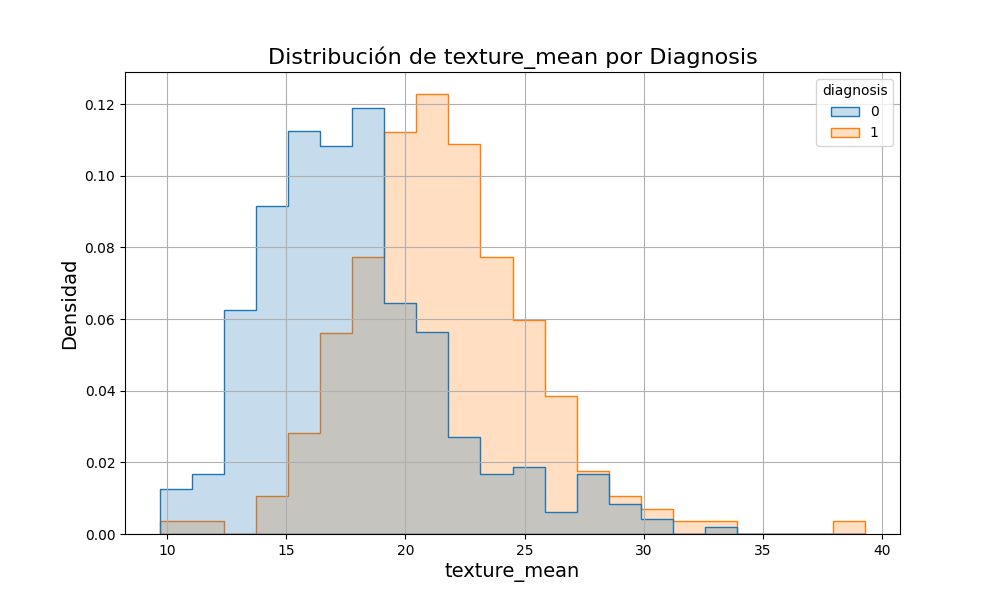
\includegraphics[width=\textwidth]{../Plots/plots_diagnosis/distribucion_texture_mean_por_diagnosis.png}

\subsection*{\underline{perimeter\_mean}}

    \begin{itemize}
	\item \textit{Descripción:} Promedio del perímetro de las células tumorales.
	\item \textit{Medición:} Longitud total de la frontera de la célula.
	\item \textit{Unidades:} Micrómetros ($\mu$m).
\end{itemize}

	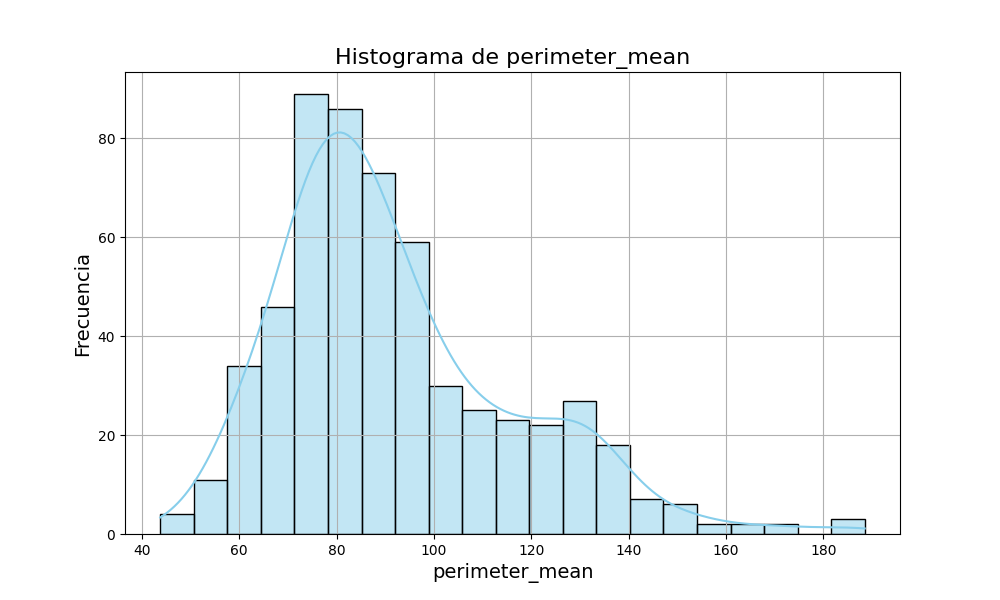
\includegraphics[width=\textwidth]{../Plots/plots_stats/perimeter_mean/histograma_perimeter_mean.png}

Histograma

\begin{itemize}
\item La distribución de\textit{perimeter mean}no es perfectamente simétrica; tiene un sesgo positivo (derecha).
\item Hay una concentración alta de valores en el extremo izquierdo, y la cola derecha es más larga, lo que indica que algunos valores elevados están arrastrando la media hacia arriba.
\item Esto refuerza la conclusión del boxplot sobre la presencia de valores atípicos altos.
\end{itemize}



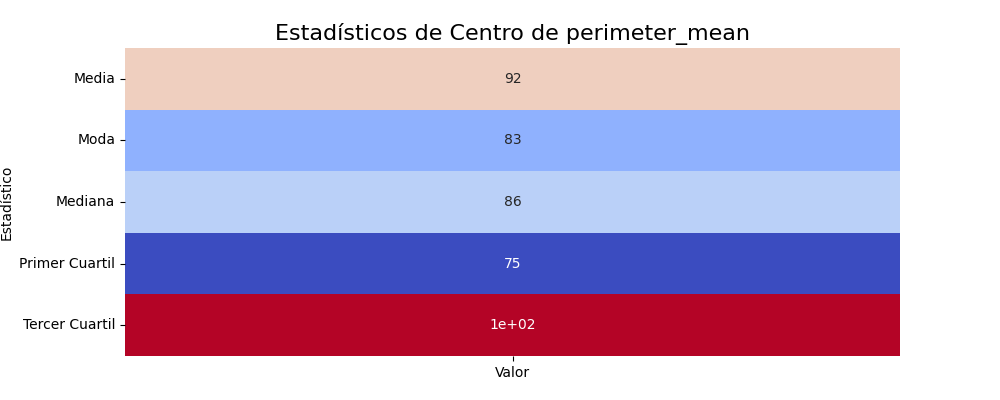
\includegraphics[width=\textwidth]{../Plots/plots_stats/perimeter_mean/estadisticas_centro_perimeter_mean.png}

Estadísticas de tendencia central

\begin{itemize}
\item La media es mayor que la mediana, confirmando el sesgo positivo observado en el histograma y el boxplot.
\item La moda parece estar en el extremo inferior, lo que indica que la mayoría de los valores son pequeños en comparación con el rango total.
\end{itemize}


\includegraphics[width=\textwidth]{../Plots/plots_stats/perimeter_mean/estadisticos_dispersión_perimeter_mean.png}

Estadísticas de dispersión

\begin{itemize}
\item La desviación estándar es alta, lo que indica que los datos están bastante dispersos.
\item El rango intercuartílico (IQR) no es excesivamente grande, pero combinado con la desviación estándar alta, refuerza la presencia de valores atípicos.
\item La varianza es elevada, lo que sugiere que los valores de\textit{perimeter mean}pueden ser bastante diferentes entre sí.
\end{itemize}


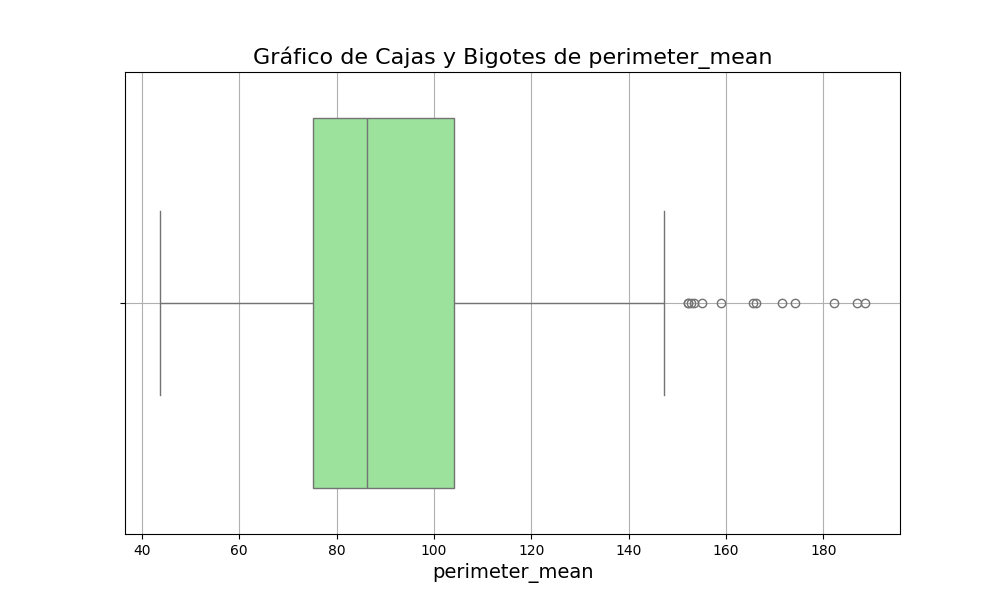
\includegraphics[width=\textwidth]{../Plots/plots_stats/perimeter_mean/boxplot_perimeter_mean.png}
Boxplot (Diagrama de caja)

\begin{itemize}
\item La caja muestra una ligera asimetría hacia la derecha, lo que indica que la distribución tiene un sesgo positivo.
\item Hay varios valores atípicos por encima del bigote superior, lo que sugiere la presencia de algunos datos extremos altos.
\item El rango intercuartílico (IQR) es moderado, lo que indica que los datos están relativamente concentrados, pero con algunos valores extremos que podrían influir en la media.
\end{itemize}


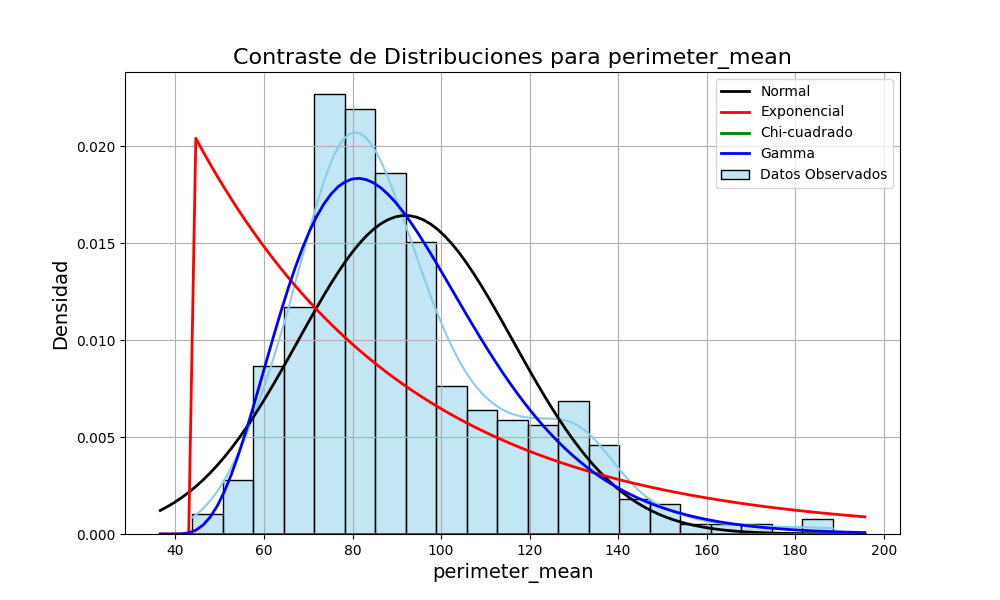
\includegraphics[width=\textwidth]{../Plots/plots_stats/perimeter_mean/distribuciones_conocidas_perimeter_mean.png}
Distribuciones conocidas

\begin{itemize}
\item La distribución de\textit{perimeter mean}no se ajusta perfectamente a una distribución normal.
\item Se observa una mejor coincidencia con una distribución asimétrica, posiblemente log-normal o gamma.
\item Esto implica que asumir normalidad en los datos podría llevar a errores en algunos análisis estadísticos.
\end{itemize}


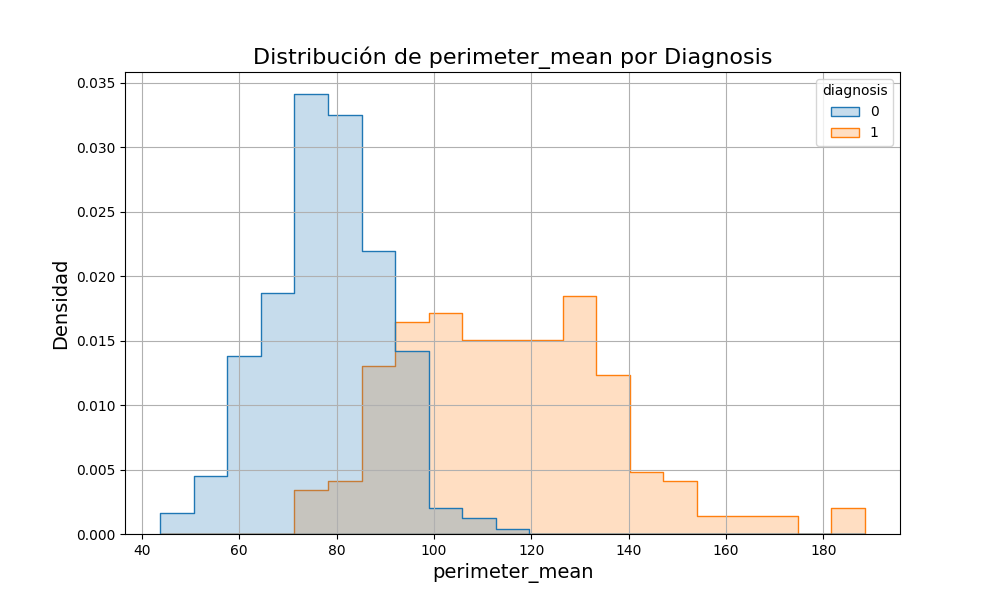
\includegraphics[width=\textwidth]{../Plots/plots_diagnosis/distribucion_perimeter_mean_por_diagnosis.png}


\subsection*{\underline{area\_mean}}

 \begin{itemize}
	\item \textit{Descripción:} Promedio del área de las células tumorales.
	\item \textit{Medición:} Área calculada a partir de la imagen digitalizada.
	\item \textit{Unidades:} Micrómetros cuadrados ($\mu$m$^2$).
\end{itemize}

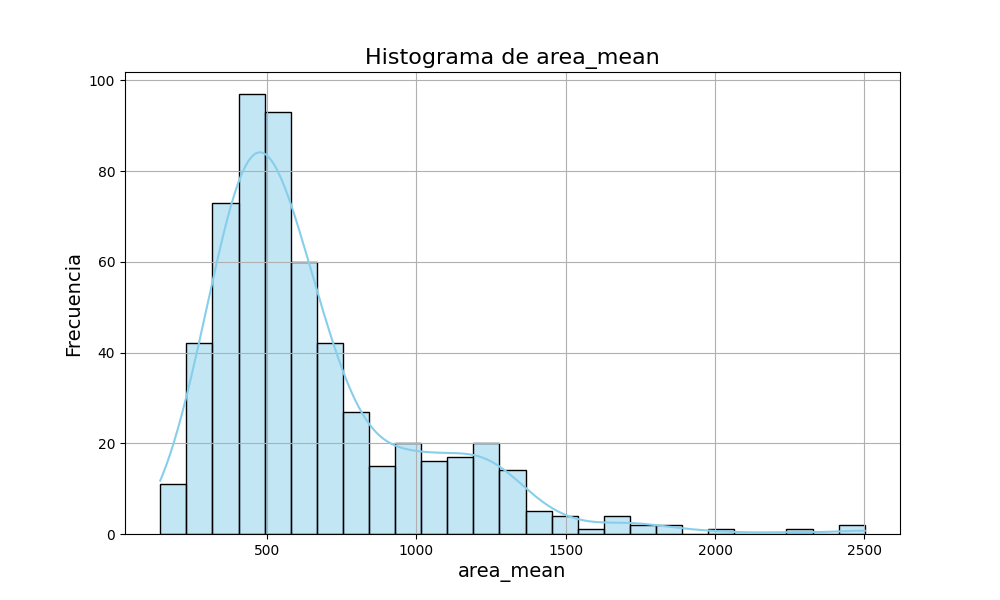
\includegraphics[width=\textwidth]{../Plots/plots_stats/area_mean/histograma_area_mean.png}

Histograma de area mean

\begin{itemize}
\item El histograma muestra una distribución unimodal (con un solo pico) y asimétrica, con una cola larga hacia la derecha. Esto indica que la mayoría de los valores de area mean están concentrados en la parte izquierda del gráfico, pero hay algunos valores más altos que se desvían de la mayoría.
\end{itemize}

Características principales:

\begin{itemize}
\item Forma:Unimodal y asimétrica, con sesgo positivo.
\item Concentración:La mayoría de los valores se encuentran en la parte izquierda del histograma.
\item Cola larga:Presencia de una cola que se extiende hacia la derecha, lo que sugiere la posible presencia de valores atípicos.
\end{itemize}

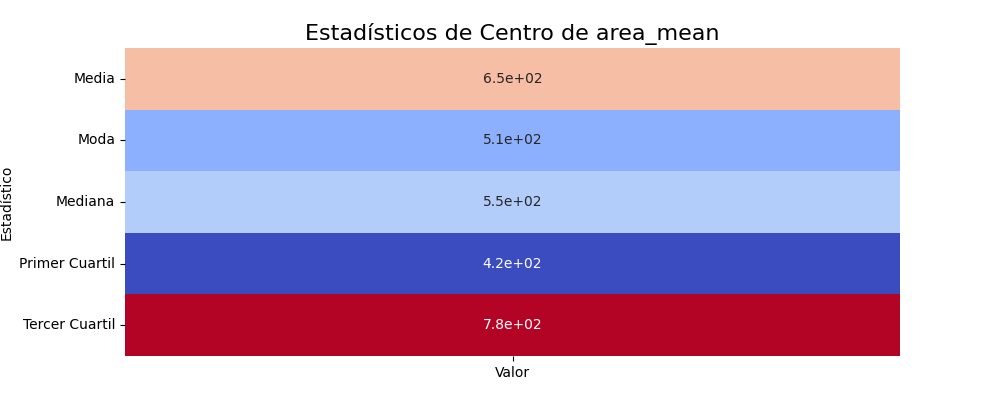
\includegraphics[width=\textwidth]{../Plots/plots_stats/area_mean/estadisticas_centro_area_mean.png}
Interpretación de estadisticas de centro de area mean

\begin{itemize}
\item Asimetría:La diferencia entre la media y la mediana (la media es mayor que la mediana) sugiere la influencia de valores atípicos en la media.
\item Concentración:La moda (510) es el valor más frecuente en el conjunto de datos.
\end{itemize}

\includegraphics[width=\textwidth]{../Plots/plots_stats/area_mean/estadisticos_dispersión_area_mean.png}
Estadísticos de Dispersión de area mean
\begin{itemize}
\item Los estadísticos de dispersión indican cuánto se dispersan los datos alrededor de su valor central.
\end{itemize}

Interpretación:

\begin{itemize}
\item Dispersión considerable:La desviación estándar y el rango relativamente altos indican una dispersión considerable de los datos alrededor de la media.
\item Variabilidad moderada:El coeficiente de variación sugiere una variabilidad moderada en relación con la media.
\end{itemize}

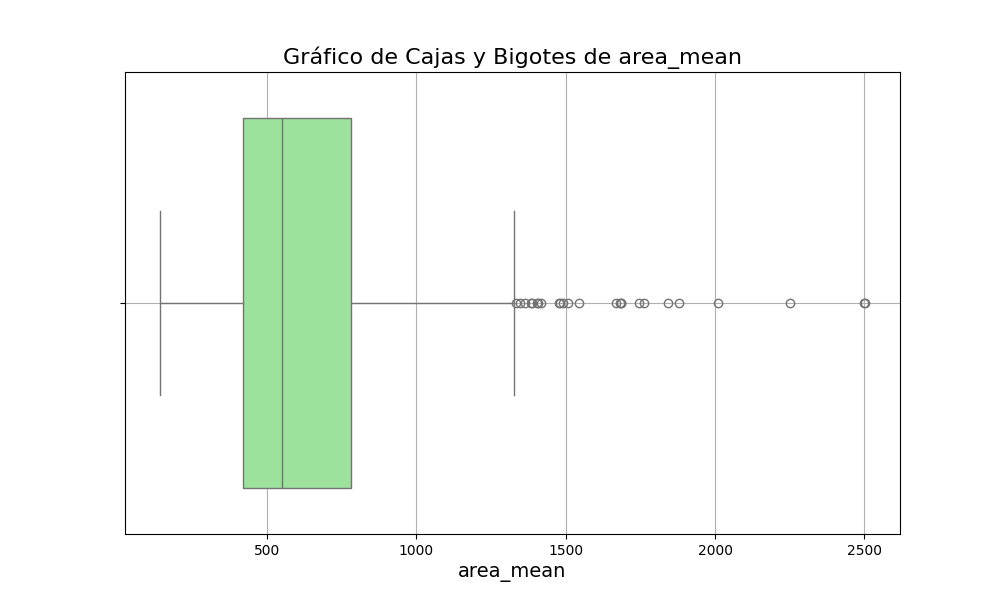
\includegraphics[width=\textwidth]{../Plots/plots_stats/area_mean/boxplot_area_mean.png}

Gráfico de Caja y Bigotes de area mean
\begin{itemize}
\item El diagrama de caja y bigotes confirma la asimetría observada en el histograma. La caja (que representa el 50% central de los datos) está sesgada hacia la izquierda, y los "bigotes" se extienden más hacia la derecha. Además, se observan varios puntos individuales a la derecha del bigote superior, lo que sugiere la presencia de valores atípicos.
\end{itemize}

Características principales:

\begin{itemize}
\item Asimetría:La caja está sesgada hacia la izquierda, lo que indica un sesgo positivo en los datos.
\item Valores atípicos:Presencia de puntos individuales fuera de los bigotes, lo que sugiere la existencia de valores atípicos.
\end{itemize}

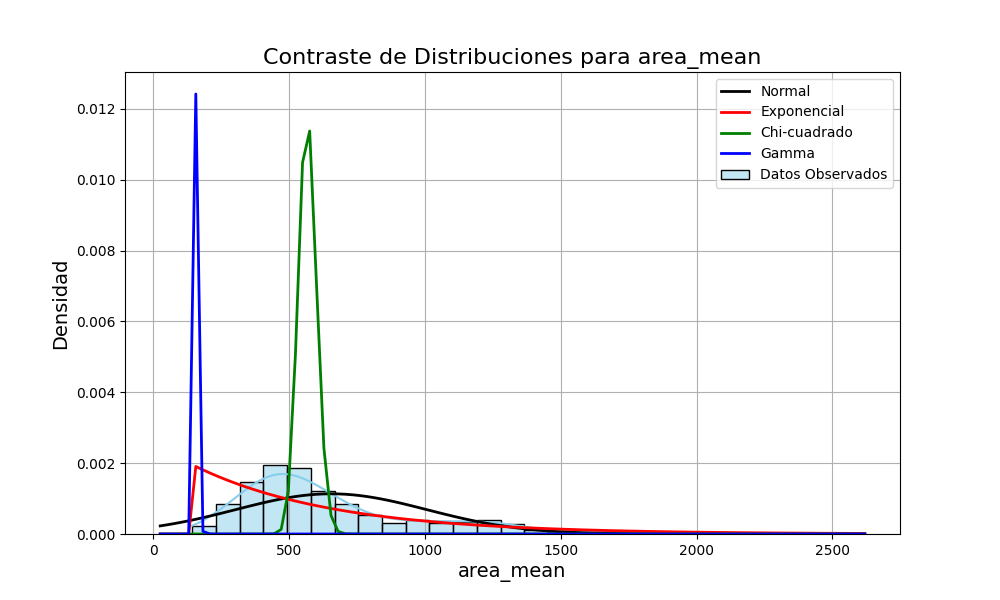
\includegraphics[width=\textwidth]{../Plots/plots_stats/area_mean/distribuciones_conocidas_area_mean.png}
Contraste de Distribuciones para area mean

\begin{itemize}
\item Este gráfico compara la distribución de los datos observados con diferentes distribuciones teóricas (Normal, Exponencial, Ji-cuadrado y Gamma).
\end{itemize}

Observaciones:

\begin{itemize}
\item Ajuste a distribución Gamma:La distribución Gamma es la que mejor se ajusta a los datos observados.
\item Asimetría:Los datos no siguen una distribución normal debido a la asimetría observada.
\end{itemize}

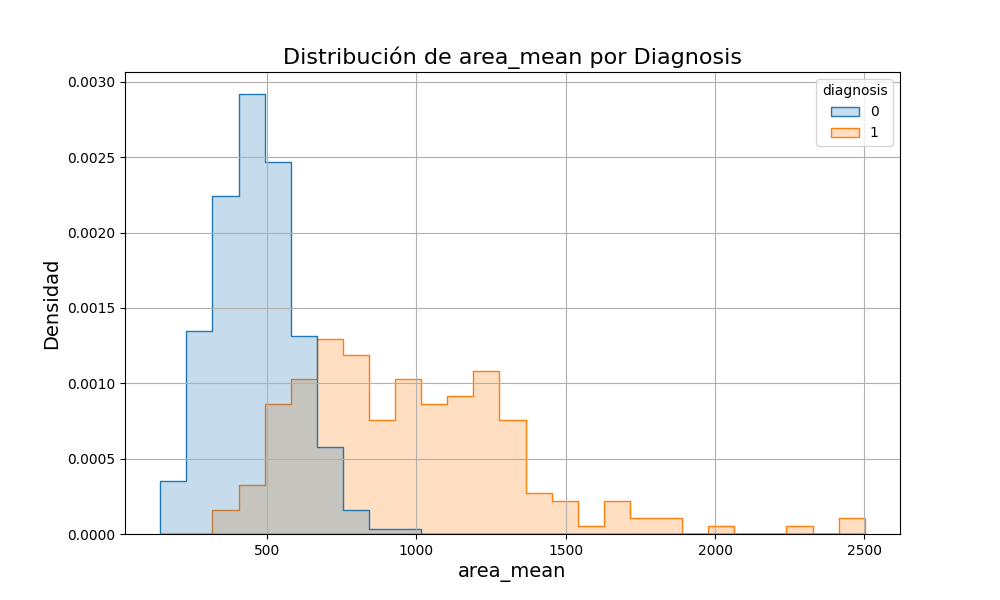
\includegraphics[width=\textwidth]{../Plots/plots_diagnosis/distribucion_area_mean_por_diagnosis.png}

\subsection*{\underline{smoothness\_mean}}

 \begin{itemize}
	\item \textit{Descripción:} Promedio de la uniformidad del contorno de las células.
	\item \textit{Medición:} Variación local de los radios en el contorno.
	\item \textit{Unidades:} Valor adimensional.
\end{itemize}

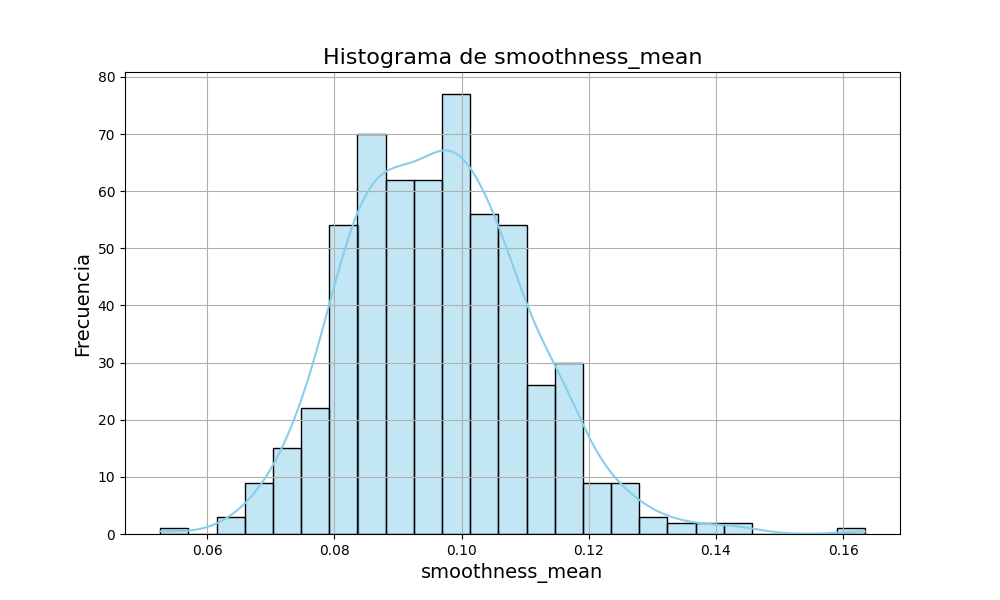
\includegraphics[width=\textwidth]{../Plots/plots_stats/smoothness_mean/histograma_smoothness_mean.png}

Histograma de smoothness mean
\begin{itemize}
\item El histograma muestra una distribución unimodal (un solo pico) y simétrica, con una forma de campana centrada alrededor de un valor cercano a 0.1. Esto indica que los valores de "smoothness_mean" se distribuyen de manera uniforme alrededor de su valor central.

Características principales

\item Forma: Unimodal y simétrica, con forma de campana.
\item Concentración: La mayoría de los valores se encuentran en el centro del histograma, alrededor de 0.1.
\item Valores centrales: No se observan valores atípicos significativos.
\end{itemize}

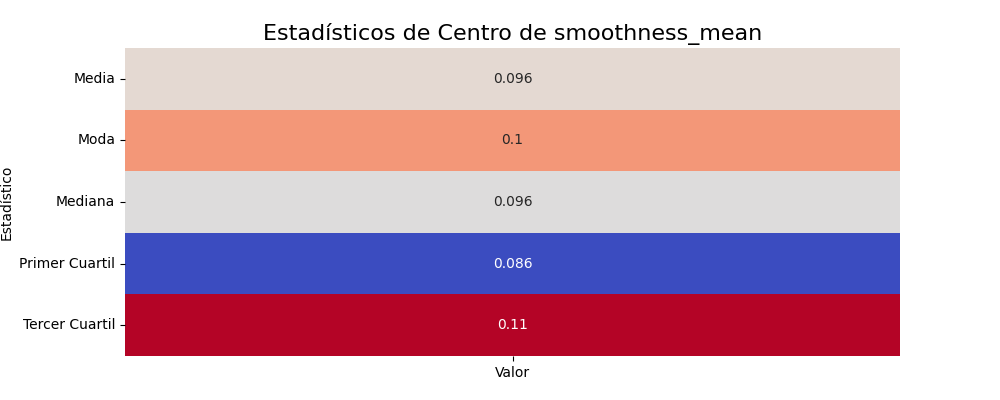
\includegraphics[width=\textwidth]{../Plots/plots_stats/smoothness_mean/estadisticas_centro_smoothness_mean.png}
Estadísticos de Centro de smoothness mean
\begin{itemize}
\item Los estadísticos de centro proporcionan información sobre la ubicación central de los datos.

\item Valores

\item Media: 0.096
\item Mediana: 0.096
\item Moda: 0.1
\item Interpretación

\item Simetría: La media y la mediana tienen valores muy similares (0.096), lo que sugiere una distribución simétrica.
\item Concentración: La moda (0.1) es muy cercana a la media y la mediana, lo que refuerza la idea de una distribución simétrica con una concentración de valores alrededor del centro.
\end{itemize}


\includegraphics[width=\textwidth]{../Plots/plots_stats/smoothness_mean/estadisticos_dispersión_smoothness_mean.png}

Estadísticos de Dispersión de smoothness mean
\begin{itemize}
\item Los estadísticos de dispersión indican cuánto se dispersan los datos alrededor de su valor central.

\item Valores

\item Desviación Estándar: 0.014
\item Rango: 0.107
\item Coeficiente de Variación: 15%
\item Interpretación

\item Dispersión moderada: La desviación estándar y el rango indican una dispersión moderada de los datos alrededor de la media.
\item Baja variabilidad: El coeficiente de variación sugiere una baja variabilidad en relación con la media.
\end{itemize}


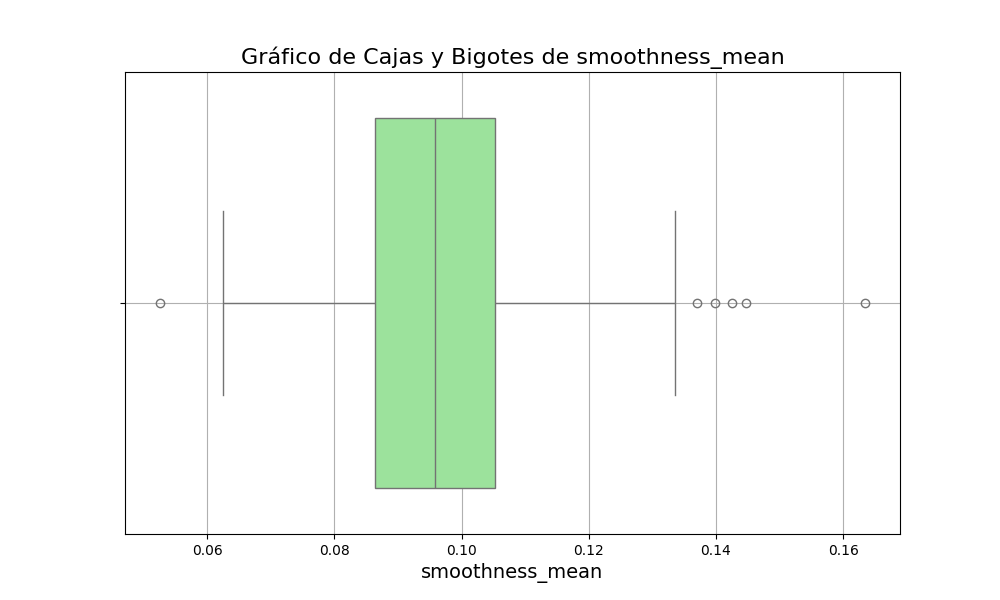
\includegraphics[width=\textwidth]{../Plots/plots_stats/smoothness_mean/boxplot_smoothness_mean.png}

Gráfico de Caja y Bigotes de smoothness mean
\begin{itemize}
\item El gráfico de caja y bigotes confirma la simetría observada en el histograma. La caja (que representa el 50 porciento central de los datos) es simétrica y los "bigotes" se extienden de manera similar hacia ambos lados. Además, no se observan puntos individuales fuera de los bigotes, lo que sugiere la ausencia de valores atípicos significativos)

Características principales

\item Simetría: La caja es simétrica, lo que indica una distribución simétrica de los datos.
\item Ausencia de valores atípicos: No se observan puntos fuera de los bigotes, lo que sugiere la ausencia de valores atípicos significativos.
\end{itemize}

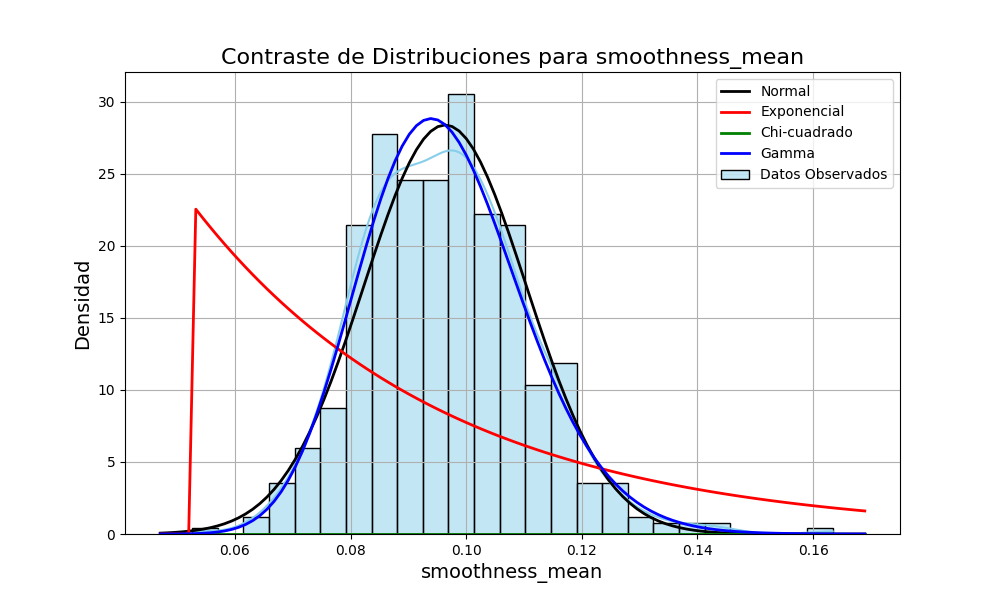
\includegraphics[width=\textwidth]{../Plots/plots_stats/smoothness_mean/distribuciones_conocidas_smoothness_mean.png}

Contraste de Distribuciones para smoothness mean
\begin{itemize}
\item Este gráfico compara la distribución observada de los datos con diferentes distribuciones teóricas (Normal, Exponencial, Chi-cuadrado y Gamma).

Observaciones

\item Ajuste de la distribución normal: La distribución normal es la que mejor se ajusta a los datos observados.
\item Simetría: Los datos siguen una distribución normal de manera bastante precisa, lo que confirma la simetría observada en las otras gráficas.
En resumen
\item La variable smoothness mean muestra una distribución simétrica, con una concentración de valores alrededor de 0.1. Esto se refleja en la similitud entre la media, la mediana y la moda, así como en la ausencia de valores atípicos en el gráfico de caja y bigotes. Los estadísticos de dispersión confirman la moderada variabilidad de los datos.
\end{itemize}


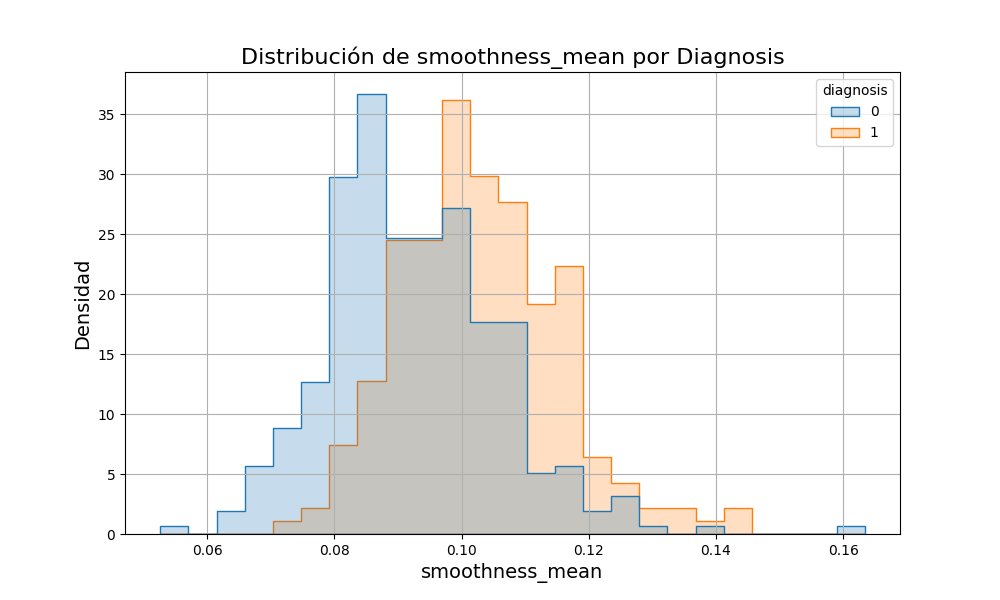
\includegraphics[width=\textwidth]{../Plots/plots_diagnosis/distribucion_smoothness_mean_por_diagnosis.png}

\subsection*{\underline{compactness\_mean}}
  \begin{itemize}
	\item \textit{Descripción:} Promedio de la compacidad de las células.
	\item \textit{Medición:} Relación entre el perímetro y el área:
	\[
	\text{Compactness} = \frac{\text{Perimeter}^2}{\text{Area}} - 1
	\]
	\item \textit{Unidades:} Valor adimensional.
\end{itemize}

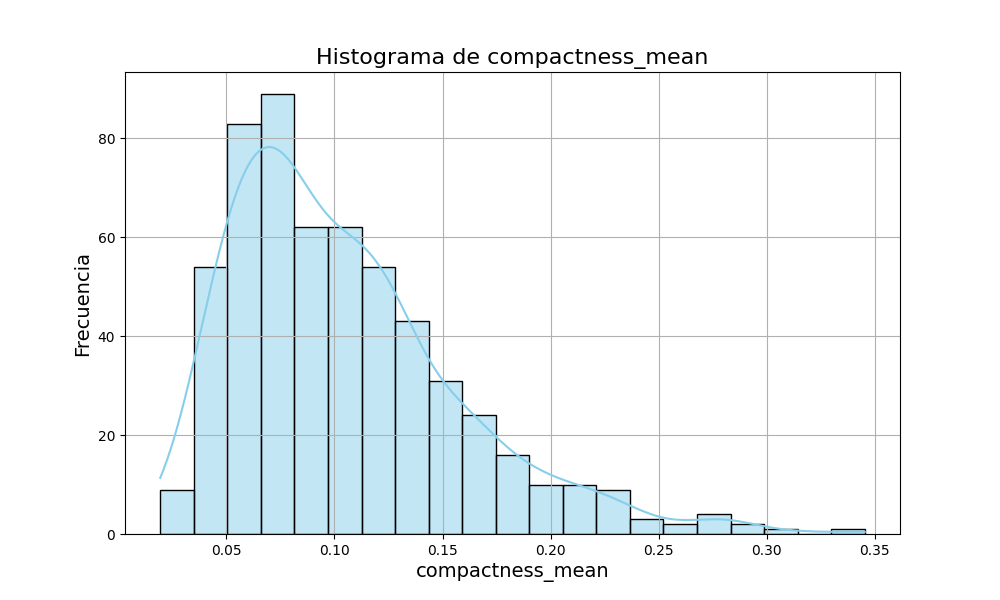
\includegraphics[width=\textwidth]{../Plots/plots_stats/compactness_mean/histograma_compactness_mean.png}

Histograma de compactness mean

\begin{itemize}
\item El histograma muestra una distribución unimodal (un solo pico) y asimétrica, con una cola larga hacia la derecha. Esto indica que la mayoría de los valores de compactness mean se concentran en la parte izquierda del gráfico, pero hay algunos valores más altos que se alejan de la mayoría.

\item Características principales

\item Forma: Unimodal y asimétrica, con sesgo positivo.
\item Concentración: La mayoría de los valores se encuentran en la parte izquierda del histograma.
\item Cola larga: Presencia de una cola que se extiende hacia la derecha, lo que sugiere la posible presencia de valores atípicos.
\end{itemize}

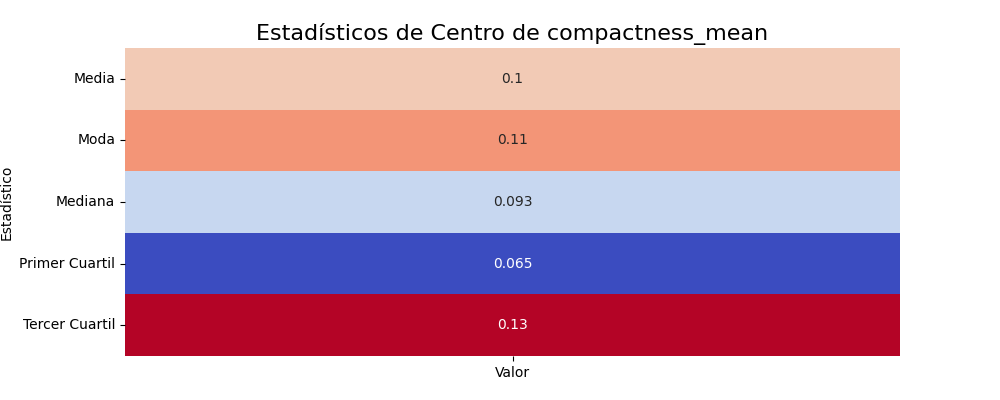
\includegraphics[width=\textwidth]{../Plots/plots_stats/compactness_mean/estadisticas_centro_compactness_mean.png}

Estadísticos de Centro de compactness mean
\begin{itemize}
\item Los estadísticos de centro proporcionan información sobre la ubicación central de los datos.
\item Valores

\item Media: 0.1
\item Mediana: 0.093
\item Moda: 0.11
\item Interpretación

\item Asimetría: La diferencia entre la media y la mediana (la media es mayor que la mediana) sugiere la influencia de los valores atípicos en la media.
\item Concentración: La moda (0.11) es el valor más frecuente en el conjunto de datos.
\end{itemize}

\includegraphics[width=\textwidth]{../Plots/plots_stats/compactness_mean/estadisticos_dispersión_compactness_mean.png}
Estadísticos de Dispersión de compactness mean
\begin{itemize}
\item Los estadísticos de dispersión indican cuánto se dispersan los datos alrededor de su valor central.

\item Valores

\item Desviación Estándar: 0.053
\item Rango: 0.331
\item Coeficiente de Variación: 51%
\item Interpretación

\item Dispersión considerable: La desviación estándar y el rango relativamente altos indican una dispersión considerable de los datos alrededor de la media.
\item Variabilidad moderada: El coeficiente de variación sugiere una variabilidad moderada en relación con la media.
\end{itemize}


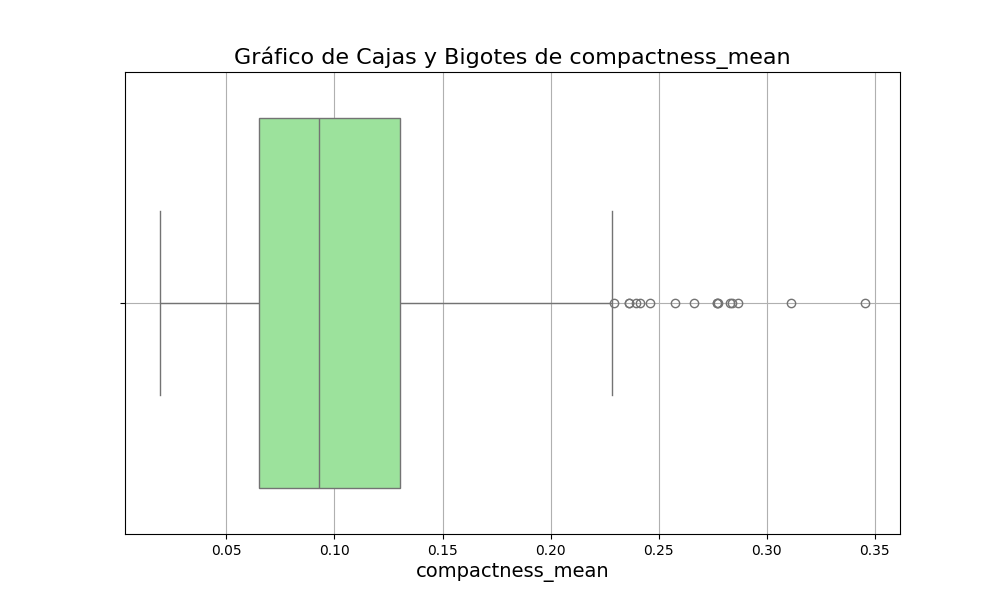
\includegraphics[width=\textwidth]{../Plots/plots_stats/compactness_mean/boxplot_compactness_mean.png}

Gráfico de Caja y Bigotes de compactness mean
\begin{itemize}
\item El gráfico de caja y bigotes confirma la asimetría observada en el histograma. La caja (que representa el 50 porciento central de los datos) está sesgada hacia la izquierda, y los "bigotes" se extienden más hacia la derecha. Además, se observan varios puntos individuales a la derecha del bigote superior, lo que sugiere la presencia de valores atípicos.
Características principales

\item Asimetría: La caja está sesgada hacia la izquierda, lo que indica un sesgo positivo en los datos.
\item Valores atípicos: Presencia de puntos individuales fuera de los bigotes, lo que sugiere la presencia de valores atípicos.
\end{itemize}

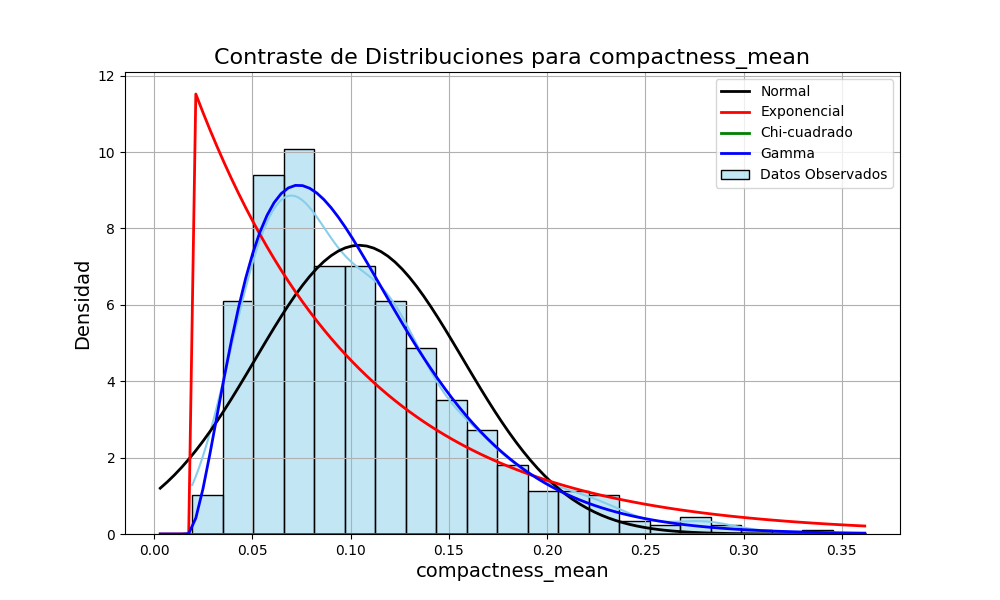
\includegraphics[width=\textwidth]{../Plots/plots_stats/compactness_mean/distribuciones_conocidas_compactness_mean.png}

Contraste de Distribuciones para compactness mean
\begin{itemize}
\item Este gráfico compara la distribución observada de los datos con diferentes distribuciones teóricas (Normal, Exponencial, Chi-cuadrado y Gamma).

\item Observaciones

\item Ajuste de la distribución Gamma: La distribución Gamma es la que mejor se ajusta a los datos observados.
\item Asimetría: Los datos no siguen una distribución normal, debido a la asimetría observada.
En resumen
\item La variable compactness mean muestra una distribución asimétrica, con una concentración de valores en la parte izquierda del histograma y una cola larga hacia la derecha. Esto se refleja en la diferencia entre la media y la mediana, así como en la presencia de valores atípicos en el gráfico de caja y bigotes. Los estadísticos de dispersión confirman la considerable variabilidad de los datos.
\end{itemize}

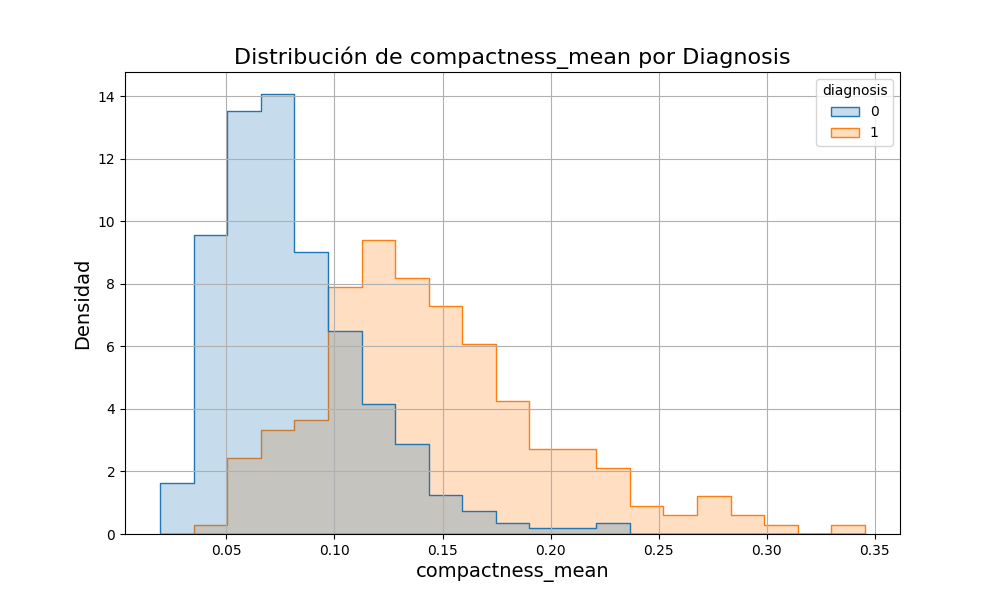
\includegraphics[width=\textwidth]{../Plots/plots_diagnosis/distribucion_compactness_mean_por_diagnosis.png}

\subsection*{\underline{symmetry\_mean}}
    \begin{itemize}
	\item \textit{Descripción:} Promedio de la simetría de las células.
	\item \textit{Medición:} Diferencia entre los radios en distintas direcciones.
	\item \textit{Unidades:} Valor adimensional.
\end{itemize}

	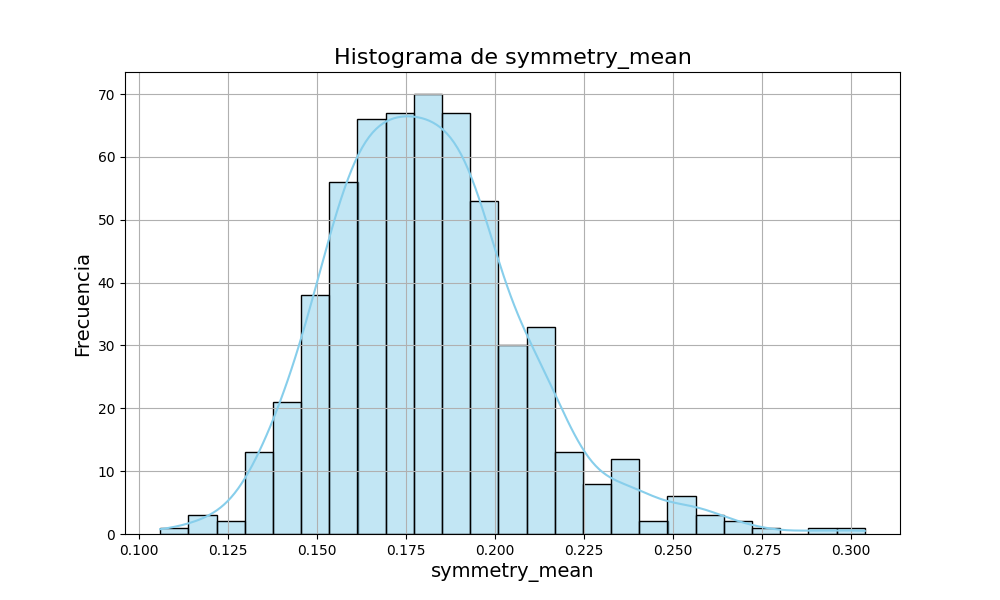
\includegraphics[width=\textwidth]{../Plots/plots_stats/symmetry_mean/histograma_symmetry_mean.png}
Histograma de symmetry mean
\begin{itemize}
\item El histograma muestra una distribución unimodal (un solo pico) y ligeramente asimétrica, con una cola larga hacia la derecha. Esto indica que la mayoría de los valores de symmetry mean se concentran en la parte izquierda del gráfico, pero hay algunos valores más altos que se alejan de la mayoría.

\item Características principales

\item Forma: Unimodal y ligeramente asimétrica, con sesgo positivo.
\item Concentración: La mayoría de los valores se encuentran en la parte izquierda del histograma.
\item Cola larga: Presencia de una cola que se extiende hacia la derecha, lo que sugiere la posible presencia de valores atípicos.
\end{itemize}

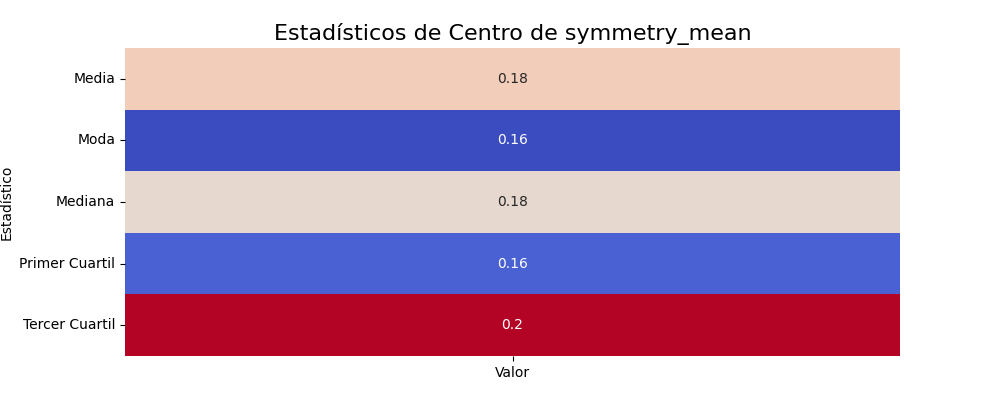
\includegraphics[width=\textwidth]{../Plots/plots_stats/symmetry_mean/estadisticas_centro_symmetry_mean.png}

Estadísticos de Centro de symmetry mean
\begin{itemize}
\item Los estadísticos de centro proporcionan información sobre la ubicación central de los datos.

\item Valores

\item Media: 0.18
\item Mediana: 0.18
\item Moda: 0.16
\item Interpretación

\item Simetría: La media y la mediana tienen valores muy similares (0.18), lo que sugiere que la distribución es bastante simétrica, aunque con una ligera asimetría.
\item Concentración: La moda (0.16) es ligeramente menor que la media y la mediana, lo que indica que la mayoría de los valores se concentran un poco por debajo del centro de la distribución.
\end{itemize}


\includegraphics[width=\textwidth]{../Plots/plots_stats/symmetry_mean/estadisticos_dispersión_symmetry_mean.png}

Estadísticos de Dispersión de symmetry mean
\begin{itemize}
\item Los estadísticos de dispersión indican cuánto se dispersan los datos alrededor de su valor central.

\item Valores

\item Desviación Estándar: 0.027
\item Rango: 0.19
\item Coeficiente de Variación: 15%
\item Interpretación

\item Dispersión moderada: La desviación estándar y el rango indican una dispersión moderada de los datos alrededor de la media.
\item Baja variabilidad: El coeficiente de variación sugiere una baja variabilidad en relación con la media.
\end{itemize}


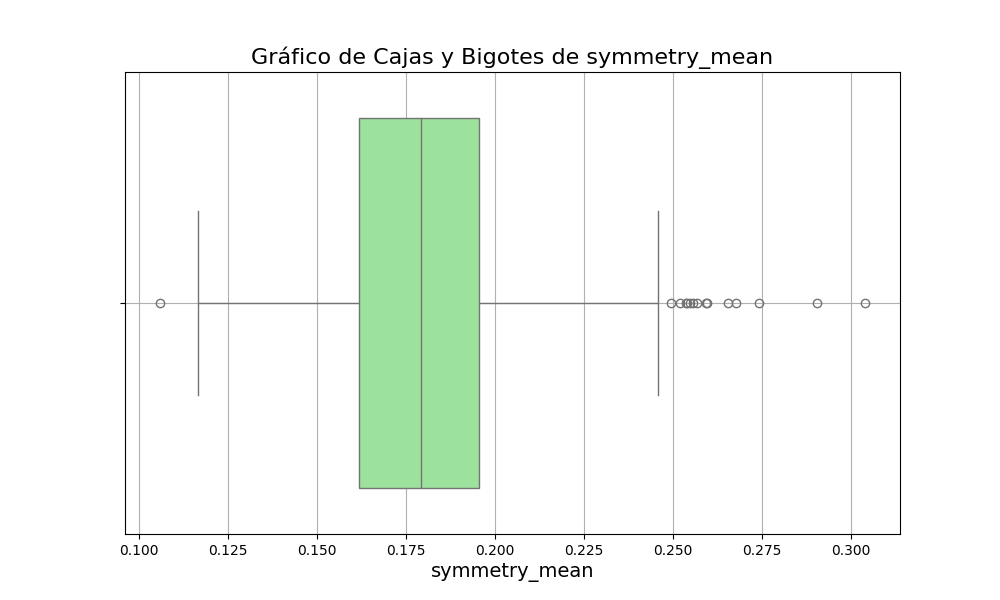
\includegraphics[width=\textwidth]{../Plots/plots_stats/symmetry_mean/boxplot_symmetry_mean.png}

Gráfico de Caja y Bigotes de symmetry mean
\begin{itemize}
\item El gráfico de caja y bigotes confirma la ligera asimetría observada en el histograma. La caja (que representa el 50 porciento central de los datos) está ligeramente sesgada hacia la izquierda, y los "bigotes" se extienden más hacia la derecha. Además, se observan varios puntos individuales a la derecha del bigote superior, lo que sugiere la presencia de valores atípicos.

Características principales

\item Asimetría: La caja está ligeramente sesgada hacia la izquierda, lo que indica un ligero sesgo positivo en los datos.
\item Valores atípicos: Presencia de puntos individuales fuera de los bigotes, lo que sugiere la presencia de valores atípicos.
\end{itemize}


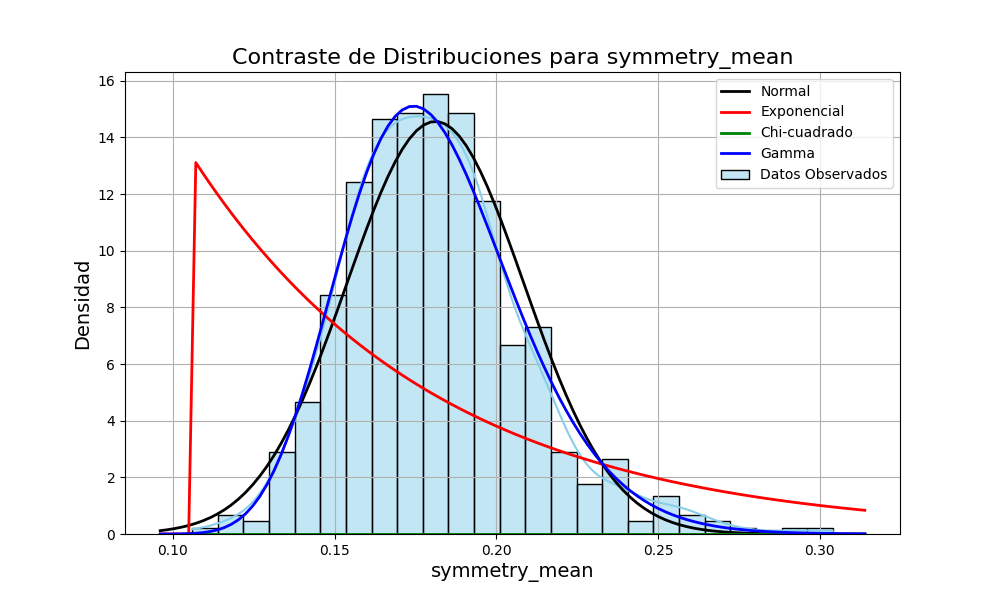
\includegraphics[width=\textwidth]{../Plots/plots_stats/symmetry_mean/distribuciones_conocidas_symmetry_mean.png}

Contraste de Distribuciones para symmetry mean
\begin{itemize}
\item Este gráfico compara la distribución observada de los datos con diferentes distribuciones teóricas (Normal, Exponencial, Chi-cuadrado y Gamma).

Observaciones

\item Ajuste de la distribución normal: La distribución normal es la que mejor se ajusta a los datos observados.
\item Ligera asimetría: Los datos no siguen una distribución normal perfecta, debido a la ligera asimetría observada.
En resumen
\item La variable symmetry mean muestra una distribución ligeramente asimétrica, con una concentración de valores en la parte izquierda del histograma y una cola larga hacia la derecha. Esto se refleja en la ligera diferencia entre la media y la mediana, así como en la presencia de valores atípicos en el gráfico de caja y bigotes. Los estadísticos de dispersión confirman la moderada variabilidad de los datos.
\end{itemize}

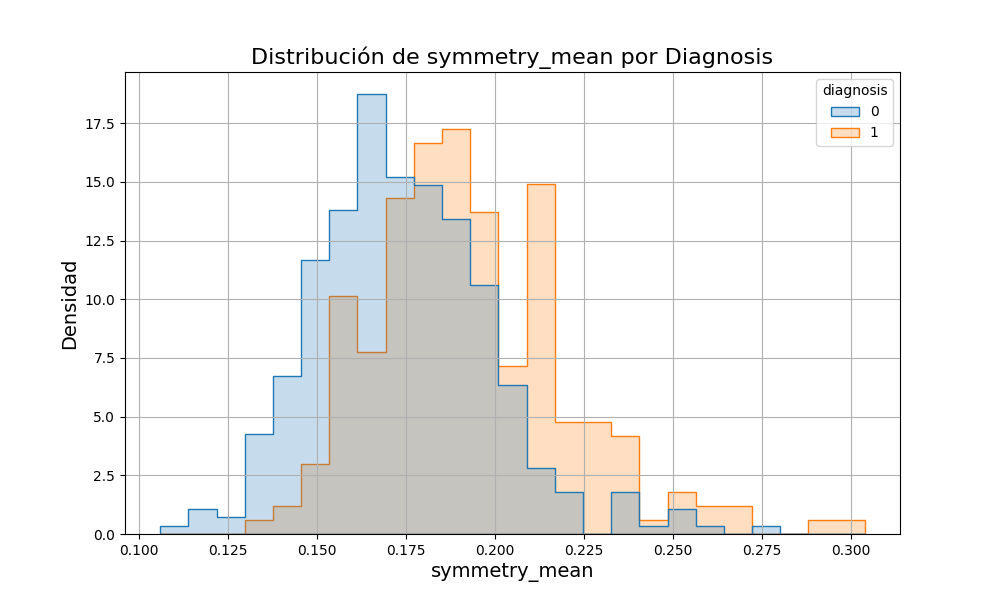
\includegraphics[width=\textwidth]{../Plots/plots_diagnosis/distribucion_symmetry_mean_por_diagnosis.png}

\newpage 

\textbf{radius\_worst, texture\_worst, perimeter\_worst, area\_worst, smoothness\_worst, compactness\_worst, symmetry\_worst}:
\begin{itemize}
	\item \textit{Descripción:} Estas variables representan los valores extremos (peores) observados en la medición de las características anteriores.
	\item \textit{Medición:} Se calculan de la misma manera que las variables \_mean pero enfocándose en los valores máximos registrados.
\end{itemize}



\subsection*{\underline{radius\_worst}}

	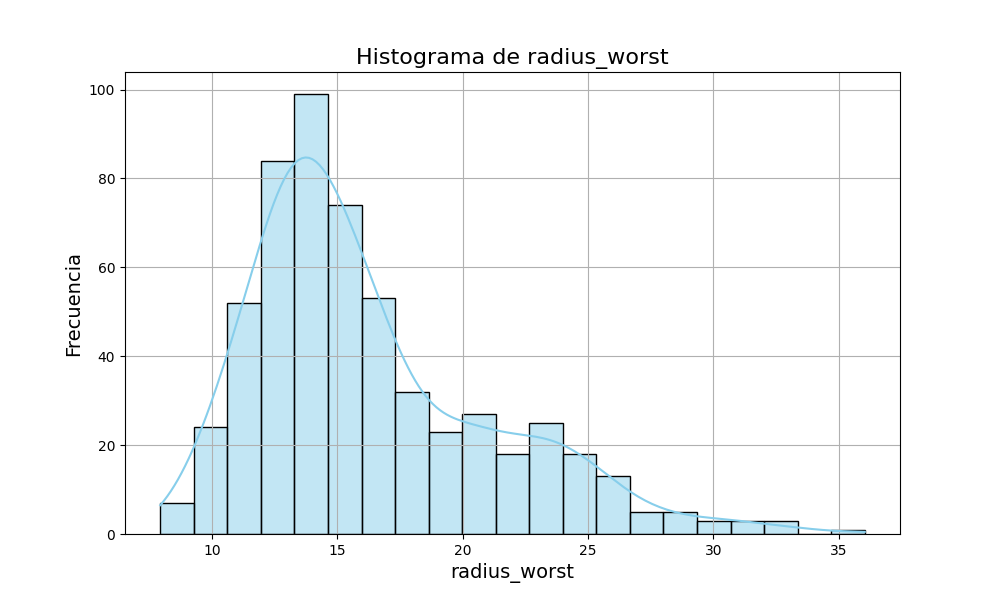
\includegraphics[width=\textwidth]{../Plots/plots_stats/radius_worst/histograma_radius_worst.png}




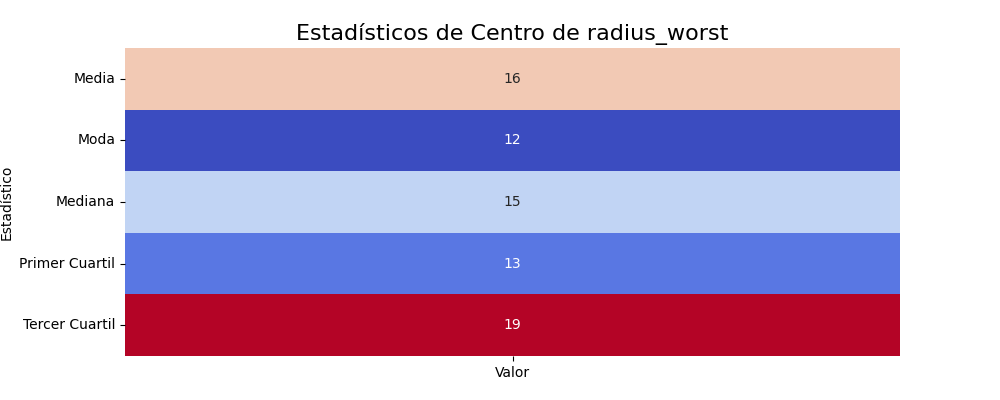
\includegraphics[width=\textwidth]{../Plots/plots_stats/radius_worst/estadisticas_centro_radius_worst.png}




\includegraphics[width=\textwidth]{../Plots/plots_stats/radius_worst/estadisticos_dispersión_radius_worst.png}



\includegraphics[width=\textwidth]{../Plots/plots_stats/radius_worst/boxplot_radius_worst.png}




\includegraphics[width=\textwidth]{../Plots/plots_stats/radius_worst/distribuciones_conocidas_radius_worst.png}

\includegraphics[width=\textwidth]{../Plots/plots_diagnosis/distribucion_radius_worst_por_diagnosis.png}


\subsection*{\underline{texture\_worst}}

	\includegraphics[width=\textwidth]{../Plots/plots_stats/texture_worst/histograma_texture_worst.png}




\includegraphics[width=\textwidth]{../Plots/plots_stats/texture_worst/estadisticas_centro_texture_worst.png}




\includegraphics[width=\textwidth]{../Plots/plots_stats/texture_worst/estadisticos_dispersión_texture_worst.png}



\includegraphics[width=\textwidth]{../Plots/plots_stats/texture_worst/boxplot_texture_worst.png}




\includegraphics[width=\textwidth]{../Plots/plots_stats/texture_worst/distribuciones_conocidas_texture_worst.png}

\includegraphics[width=\textwidth]{../Plots/plots_diagnosis/distribucion_texture_worst_por_diagnosis.png}

\subsection*{\underline{perimeter\_worst}}

	\includegraphics[width=\textwidth]{../Plots/plots_stats/perimeter_worst/histograma_perimeter_worst.png}




\includegraphics[width=\textwidth]{../Plots/plots_stats/perimeter_worst/estadisticas_centro_perimeter_worst.png}




\includegraphics[width=\textwidth]{../Plots/plots_stats/perimeter_worst/estadisticos_dispersión_perimeter_worst.png}



\includegraphics[width=\textwidth]{../Plots/plots_stats/perimeter_worst/boxplot_perimeter_worst.png}




\includegraphics[width=\textwidth]{../Plots/plots_stats/perimeter_worst/distribuciones_conocidas_perimeter_worst.png}

\includegraphics[width=\textwidth]{../Plots/plots_diagnosis/distribucion_perimeter_worst_por_diagnosis.png}

\subsection*{\underline{area\_worst}}

	\includegraphics[width=\textwidth]{../Plots/plots_stats/area_worst/histograma_area_worst.png}




\includegraphics[width=\textwidth]{../Plots/plots_stats/area_worst/estadisticas_centro_area_worst.png}




\includegraphics[width=\textwidth]{../Plots/plots_stats/area_worst/estadisticos_dispersión_area_worst.png}



\includegraphics[width=\textwidth]{../Plots/plots_stats/area_worst/boxplot_area_worst.png}




\includegraphics[width=\textwidth]{../Plots/plots_stats/area_worst/distribuciones_conocidas_area_worst.png}

\includegraphics[width=\textwidth]{../Plots/plots_diagnosis/distribucion_area_worst_por_diagnosis.png}

\subsection*{\underline{smoothness\_worst}}

	\includegraphics[width=\textwidth]{../Plots/plots_stats/smoothness_worst/histograma_smoothness_worst.png}




\includegraphics[width=\textwidth]{../Plots/plots_stats/smoothness_worst/estadisticas_centro_smoothness_worst.png}




\includegraphics[width=\textwidth]{../Plots/plots_stats/smoothness_worst/estadisticos_dispersión_smoothness_worst.png}



\includegraphics[width=\textwidth]{../Plots/plots_stats/smoothness_worst/boxplot_smoothness_worst.png}




\includegraphics[width=\textwidth]{../Plots/plots_stats/smoothness_worst/distribuciones_conocidas_smoothness_worst.png}

\includegraphics[width=\textwidth]{../Plots/plots_diagnosis/distribucion_smoothness_worst_por_diagnosis.png}

\subsection*{\underline{compactness\_worst}}

	\includegraphics[width=\textwidth]{../Plots/plots_stats/smoothness_worst/histograma_smoothness_worst.png}




\includegraphics[width=\textwidth]{../Plots/plots_stats/smoothness_worst/estadisticas_centro_smoothness_worst.png}




\includegraphics[width=\textwidth]{../Plots/plots_stats/smoothness_worst/estadisticos_dispersión_smoothness_worst.png}



\includegraphics[width=\textwidth]{../Plots/plots_stats/smoothness_worst/boxplot_smoothness_worst.png}




\includegraphics[width=\textwidth]{../Plots/plots_stats/smoothness_worst/distribuciones_conocidas_smoothness_worst.png}

\includegraphics[width=\textwidth]{../Plots/plots_diagnosis/distribucion_smoothness_worst_por_diagnosis.png}

\subsection*{\underline{symmetry\_worst}}

	\includegraphics[width=\textwidth]{../Plots/plots_stats/symmetry_worst/histograma_symmetry_worst.png}




\includegraphics[width=\textwidth]{../Plots/plots_stats/symmetry_worst/estadisticas_centro_symmetry_worst.png}




\includegraphics[width=\textwidth]{../Plots/plots_stats/symmetry_worst/estadisticos_dispersión_symmetry_worst.png}



\includegraphics[width=\textwidth]{../Plots/plots_stats/symmetry_worst/boxplot_symmetry_worst.png}




\includegraphics[width=\textwidth]{../Plots/plots_stats/symmetry_worst/distribuciones_conocidas_symmetry_worst.png}

\includegraphics[width=\textwidth]{../Plots/plots_diagnosis/distribucion_symmetry_worst_por_diagnosis.png}


\newpage

\section{Análisis de la distribución}

\subsection{Pruebas de Normalidad}

\subsection*{Kolmogorov-Smirnov}
\includegraphics[width=\textwidth]{../Plots/resumen_normalidad.png}

\subsection*{Shapiro-Wilk}
\includegraphics[width=\textwidth]{../Plots/resumen_shapiro_wilk.png}

\subsection*{Anderson-Darling}
\includegraphics[width=\textwidth]{../Plots/resumen_anderson_darling.png}


\subsection{Estimación de parámetros}

\subsubsection{texture\_mean}

\textbf{Estimación Puntual}

\textbf{Estimación por Intervalos}


\subsubsection{smoothness\_mean}

\textbf{Estimación Puntual}

\textbf{Estimación por Intervalos}


\subsubsection{symmetry\_mean}

\textbf{Estimación Puntual}

\textbf{Estimación por Intervalos}


\subsubsection{texture\_worst}

\textbf{Estimación Puntual}

\textbf{Estimación por Intervalos}


\subsubsection{smoothness\_worst}

\textbf{Estimación Puntual}

\textbf{Estimación por Intervalos}


\subsubsection{diagnosis}

\textbf{Estimación Puntual}

\textbf{Estimación por Intervalos}


\subsection{Pruebas de Hipótesis}

\subsubsection{Pruebas de Hipótesis para una población}

\textbf{Ejemplo 1: Media de una población conocida}\\

Se desea verificar si la media de la variable \textit{texture\_mean} es igual a 20. 

\begin{itemize}
	\item \textbf{Hipótesis nula} (\(H_0\)): \(\mu = 20\)
	\item \textbf{Hipótesis alternativa} (\(H_a\)): \(\mu \neq 20\)
\end{itemize}

\textbf{Prueba}: Estadístico \( Z = \frac{\bar{x} - \mu}{\sigma / \sqrt{n}} \)\\

\textbf{Ejemplo 2: Proporción de una población}\\

Se desea verificar si la proporción de diagnósticos de tipo \textit{Maligno} es mayor al 50\%.

\begin{itemize}
	\item \textbf{Hipótesis nula} (\(H_0\)): \(p = 0.5\)
	\item \textbf{Hipótesis alternativa} (\(H_a\)): \(p > 0.5\)
\end{itemize}

\textbf{Prueba}: Estadístico \( Z = \frac{\hat{p} - p}{\sqrt{\frac{p(1-p)}{n}}} \)\\

\textbf{Ejemplo 3: Varianza de una población}\\

Se desea verificar si la varianza de la variable \textit{symmetry\_mean} es igual a 0.001. 

\begin{itemize}
	\item \textbf{Hipótesis nula} (\(H_0\)): \(\sigma^2 = 0.001\)
	\item \textbf{Hipótesis alternativa} (\(H_a\)): \(\sigma^2 \neq 0.001\)
\end{itemize}

\textbf{Prueba}: Estadístico \(\chi^2 = \frac{(n-1)S^2}{\sigma^2}\)\\
\textbf{Ejemplo 4: Media de una población con varianza desconocida}\\

Se desea verificar si la media de la variable \textit{texture\_worst} es mayor a 20.(Varianza desconocida)

\begin{itemize}
	\item \textbf{Hipótesis nula} (\(H_0\)): \(\mu \leq 20\)
	\item \textbf{Hipótesis alternativa} (\(H_a\)): \(\mu > 20\)
\end{itemize}

\textbf{Prueba}: Estadístico \( t = \frac{\bar{x} - \mu}{\sigma / \sqrt{n}} \)\\


\subsubsection{Pruebas de Hipótesis para dos poblaciones}

\textbf{Ejemplo 1: Igualdad de medias}

Se desea verificar si la media de la variable \textit{smoothness\_worst} es igual en los grupos \textit{Maligno} y \textit{Benigno}.(Varianzas Desconocidas).
Primero efectuar prueba para saber si son iguales o diferentes.

\begin{itemize}
	\item \textbf{Hipótesis nula} (\(H_0\)): \(\mu_1 = \mu_2\)
	\item \textbf{Hipótesis alternativa} (\(H_a\)): \(\mu_1 \neq \mu_2\)
\end{itemize}

\textbf{Prueba}: \(t = \frac{(\bar{x}_1 - \bar{x}_2)}{\sqrt{s_1^2/n_1 + s_2^2/n_2}}\)\\

\textbf{Ejemplo 2: Igualdad de proporciones}\\

Se desea verificar si la proporción de diagnósticos malignos es diferente entre dos grupos(a decidir todavía).

\begin{itemize}
	\item \textbf{Hipótesis nula} (\(H_0\)): \(p_1 = p_2\)
	\item \textbf{Hipótesis alternativa} (\(H_a\)): \(p_1 \neq p_2\)
\end{itemize}

\textbf{Prueba}: \(Z = \frac{(\hat{p}_1 - \hat{p}_2)}{\sqrt{\hat{p}(1-\hat{p})(1/n_1 + 1/n_2)}}\), donde \(\hat{p}\) es la proporción conjunta.\\

\textbf{Ejemplo 3: Igualdad de varianzas}\\

Se desea verificar si la varianza de la variable \textit{symmetry\_mean} es igual en los grupos \textit{Maligno} y \textit{Benigno}.

\begin{itemize}
	\item \textbf{Hipótesis nula} (\(H_0\)): \(\sigma_1^2 = \sigma_2^2\)
	\item \textbf{Hipótesis alternativa} (\(H_a\)): \(\sigma_1^2 \neq \sigma_2^2\)
\end{itemize}

\textbf{Prueba}: \(F = \frac{s_1^2}{s_2^2}\)


\newpage

\section{Correlación e Independencia}
\subsection{Correlación}
	\includegraphics[width = \textwidth]{../Plots/plots_corr/corr_matrix/matriz_correlacion_pearson.png}

	\includegraphics[width = \textwidth]{../Plots/plots_corr/corr_matrix/matriz_correlacion_spearman.png}

	De acuerdo a los resultados obtenidos se realizará un análisis más detallado de las variables con mayor correlación.

\subsubsection{area\_mean\_vs\_area\_worst}
	\includegraphics[width = \textwidth]{../Plots/plots_corr/area_mean_vs_area_worst/coeficiente_correlacion_area_mean_vs_area_worst.png}
	\includegraphics[width = \textwidth]{../Plots/plots_corr/area_mean_vs_area_worst/dispersión_area_mean_vs_area_worst.png}
	\includegraphics[width = \textwidth]{../Plots/plots_corr/area_mean_vs_area_worst/regresion_area_mean_vs_area_worst.png}
\subsubsection{area\_mean\_vs\_perimeter\_worst}
	\includegraphics[width = \textwidth]{../Plots/plots_corr/area_mean_vs_perimeter_worst/coeficiente_correlacion_area_mean_vs_perimeter_worst.png}
	\includegraphics[width = \textwidth]{../Plots/plots_corr/area_mean_vs_perimeter_worst/dispersión_area_mean_vs_perimeter_worst.png}
	\includegraphics[width = \textwidth]{../Plots/plots_corr/area_mean_vs_perimeter_worst/regresion_area_mean_vs_perimeter_worst.png}
\subsubsection{area\_mean\_vs\_radius\_worst}
	\includegraphics[width = \textwidth]{../Plots/plots_corr/area_mean_vs_radius_worst/coeficiente_correlacion_area_mean_vs_radius_worst.png}
	\includegraphics[width = \textwidth]{../Plots/plots_corr/area_mean_vs_radius_worst/dispersión_area_mean_vs_radius_worst.png}
	\includegraphics[width = \textwidth]{../Plots/plots_corr/area_mean_vs_radius_worst/regresion_area_mean_vs_radius_worst.png}
\subsection{compactness\_mean\_vs\_compactness\_worst}
    \includegraphics[width = \textwidth]{../Plots/plots_corr/compactness_mean_vs_compactness_worst/coeficiente_correlacion_compactness_mean_vs_compactness_worst.png}
    \includegraphics[width = \textwidth]{../Plots/plots_corr/compactness_mean_vs_compactness_worst/dispersión_compactness_mean_vs_compactness_worst.png}
    \includegraphics[width = \textwidth]{../Plots/plots_corr/compactness_mean_vs_compactness_worst/regresion_compactness_mean_vs_compactness_worst.png}
\subsection{diagnosis\_vs\_area\_mean}
    \includegraphics[width = \textwidth]{../Plots/plots_corr/diagnosis_vs_area_mean/coeficiente_correlacion_diagnosis_vs_area_mean.png}
    \includegraphics[width = \textwidth]{../Plots/plots_corr/diagnosis_vs_area_mean/dispersión_diagnosis_vs_area_mean.png}
    \includegraphics[width = \textwidth]{../Plots/plots_corr/diagnosis_vs_area_mean/chi_cuadrado_diagnosis_vs_area_mean.png}
\subsection{diagnosis\_vs\_area\_worst}
    \includegraphics[width = \textwidth]{../Plots/plots_corr/diagnosis_vs_area_worst/coeficiente_correlacion_diagnosis_vs_area_worst.png}
    \includegraphics[width = \textwidth]{../Plots/plots_corr/diagnosis_vs_area_worst/dispersión_diagnosis_vs_area_worst.png}
    \includegraphics[width = \textwidth]{../Plots/plots_corr/diagnosis_vs_area_worst/chi_cuadrado_diagnosis_vs_area_worst.png}
\subsection{diagnosis\_vs\_perimeter\_mean}
    \includegraphics[width = \textwidth]{../Plots/plots_corr/diagnosis_vs_perimeter_mean/coeficiente_correlacion_diagnosis_vs_perimeter_mean.png}
    \includegraphics[width = \textwidth]{../Plots/plots_corr/diagnosis_vs_perimeter_mean/dispersión_diagnosis_vs_perimeter_mean.png}
    \includegraphics[width = \textwidth]{../Plots/plots_corr/diagnosis_vs_perimeter_mean/chi_cuadrado_diagnosis_vs_perimeter_mean.png}
\subsection{diagnosis\_vs\_perimeter\_worst}
    \includegraphics[width = \textwidth]{../Plots/plots_corr/diagnosis_vs_perimeter_worst/coeficiente_correlacion_diagnosis_vs_perimeter_worst.png}
    \includegraphics[width = \textwidth]{../Plots/plots_corr/diagnosis_vs_perimeter_worst/dispersión_diagnosis_vs_perimeter_worst.png}
    \includegraphics[width = \textwidth]{../Plots/plots_corr/diagnosis_vs_perimeter_worst/chi_cuadrado_diagnosis_vs_perimeter_worst.png}
\subsection{diagnosis\_vs\_radius\_mean}
    \includegraphics[width = \textwidth]{../Plots/plots_corr/diagnosis_vs_radius_mean/coeficiente_correlacion_diagnosis_vs_radius_mean.png}
    \includegraphics[width = \textwidth]{../Plots/plots_corr/diagnosis_vs_radius_mean/dispersión_diagnosis_vs_radius_mean.png}
    \includegraphics[width = \textwidth]{../Plots/plots_corr/diagnosis_vs_radius_mean/chi_cuadrado_diagnosis_vs_radius_mean.png}
\subsection{diagnosis\_vs\_radius\_worst}
    \includegraphics[width = \textwidth]{../Plots/plots_corr/diagnosis_vs_radius_worst/coeficiente_correlacion_diagnosis_vs_radius_worst.png}
    \includegraphics[width = \textwidth]{../Plots/plots_corr/diagnosis_vs_radius_worst/dispersión_diagnosis_vs_radius_worst.png}
    \includegraphics[width = \textwidth]{../Plots/plots_corr/diagnosis_vs_radius_worst/chi_cuadrado_diagnosis_vs_radius_worst.png}
\subsection{perimeter\_mean\_vs\_area\_worst}
    \includegraphics[width = \textwidth]{../Plots/plots_corr/perimeter_mean_vs_area_worst/coeficiente_correlacion_perimeter_mean_vs_area_worst.png}
    \includegraphics[width = \textwidth]{../Plots/plots_corr/perimeter_mean_vs_area_worst/dispersión_perimeter_mean_vs_area_worst.png}
    \includegraphics[width = \textwidth]{../Plots/plots_corr/perimeter_mean_vs_area_worst/chi_cuadrado_perimeter_mean_vs_area_worst.png}
\subsection{perimeter\_mean\_vs\_area\_mean}
    \includegraphics[width = \textwidth]{../Plots/plots_corr/perimeter_mean_vs_area_mean/coeficiente_correlacion_perimeter_mean_vs_area_mean.png}
    \includegraphics[width = \textwidth]{../Plots/plots_corr/perimeter_mean_vs_area_mean/dispersión_perimeter_mean_vs_area_mean.png}
    \includegraphics[width = \textwidth]{../Plots/plots_corr/perimeter_mean_vs_area_mean/chi_cuadrado_perimeter_mean_vs_area_mean.png}
\subsection{perimeter\_mean\_vs\_perimeter\_worst}
    \includegraphics[width = \textwidth]{../Plots/plots_corr/perimeter_mean_vs_perimeter_worst/coeficiente_correlacion_perimeter_mean_vs_perimeter_worst.png}
    \includegraphics[width = \textwidth]{../Plots/plots_corr/perimeter_mean_vs_perimeter_worst/dispersión_perimeter_mean_vs_perimeter_worst.png}
    \includegraphics[width = \textwidth]{../Plots/plots_corr/perimeter_mean_vs_perimeter_worst/regresion_perimeter_mean_vs_perimeter_worst.png}
\subsection{perimeter\_mean\_vs\_radius\_worst}
    \includegraphics[width = \textwidth]{../Plots/plots_corr/perimeter_mean_vs_radius_worst/coeficiente_correlacion_perimeter_mean_vs_radius_worst.png}
    \includegraphics[width = \textwidth]{../Plots/plots_corr/perimeter_mean_vs_radius_worst/dispersión_perimeter_mean_vs_radius_worst.png}
    \includegraphics[width = \textwidth]{../Plots/plots_corr/perimeter_mean_vs_radius_worst/regresion_perimeter_mean_vs_radius_worst.png}
\subsection{perimeter\_worst\_vs\_area\_worst}
    \includegraphics[width = \textwidth]{../Plots/plots_corr/perimeter_worst_vs_area_worst/coeficiente_correlacion_perimeter_worst_vs_area_worst.png}
    \includegraphics[width = \textwidth]{../Plots/plots_corr/perimeter_worst_vs_area_worst/dispersión_perimeter_worst_vs_area_worst.png}
    \includegraphics[width = \textwidth]{../Plots/plots_corr/perimeter_worst_vs_area_worst/chi_cuadrado_perimeter_worst_vs_area_worst.png}
\subsection{radius\_mean\_vs\_area\_mean}
    \includegraphics[width = \textwidth]{../Plots/plots_corr/radius_mean_vs_area_mean/coeficiente_correlacion_radius_mean_vs_area_mean.png}
    \includegraphics[width = \textwidth]{../Plots/plots_corr/radius_mean_vs_area_mean/dispersión_radius_mean_vs_area_mean.png}
    \includegraphics[width = \textwidth]{../Plots/plots_corr/radius_mean_vs_area_mean/chi_cuadrado_radius_mean_vs_area_mean.png}
\subsection{radius\_mean\_vs\_area\_worst}
    \includegraphics[width = \textwidth]{../Plots/plots_corr/radius_mean_vs_area_worst/coeficiente_correlacion_radius_mean_vs_area_worst.png}
    \includegraphics[width = \textwidth]{../Plots/plots_corr/radius_mean_vs_area_worst/dispersión_radius_mean_vs_area_worst.png}
    \includegraphics[width = \textwidth]{../Plots/plots_corr/radius_mean_vs_area_worst/chi_cuadrado_radius_mean_vs_area_worst.png}
\subsection{radius\_mean\_vs\_perimeter\_mean}
    \includegraphics[width = \textwidth]{../Plots/plots_corr/radius_mean_vs_perimeter_mean/coeficiente_correlacion_radius_mean_vs_perimeter_mean.png}
    \includegraphics[width = \textwidth]{../Plots/plots_corr/radius_mean_vs_perimeter_mean/dispersión_radius_mean_vs_perimeter_mean.png}
    \includegraphics[width = \textwidth]{../Plots/plots_corr/radius_mean_vs_perimeter_mean/regresion_radius_mean_vs_perimeter_mean.png}
\subsection{radius\_mean\_vs\_perimeter\_worst}
    \includegraphics[width = \textwidth]{../Plots/plots_corr/radius_mean_vs_perimeter_worst/coeficiente_correlacion_radius_mean_vs_perimeter_worst.png}
    \includegraphics[width = \textwidth]{../Plots/plots_corr/radius_mean_vs_perimeter_worst/dispersión_radius_mean_vs_perimeter_worst.png}
    \includegraphics[width = \textwidth]{../Plots/plots_corr/radius_mean_vs_perimeter_worst/regresion_radius_mean_vs_perimeter_worst.png}
\subsection{radius\_mean\_vs\_radius\_worst}
    \includegraphics[width = \textwidth]{../Plots/plots_corr/radius_mean_vs_radius_worst/coeficiente_correlacion_radius_mean_vs_radius_worst.png}
    \includegraphics[width = \textwidth]{../Plots/plots_corr/radius_mean_vs_radius_worst/dispersión_radius_mean_vs_radius_worst.png}
    \includegraphics[width = \textwidth]{../Plots/plots_corr/radius_mean_vs_radius_worst/regresion_radius_mean_vs_radius_worst.png}
\subsection{radius\_worst\_vs\_area\_worst}
    \includegraphics[width = \textwidth]{../Plots/plots_corr/radius_worst_vs_area_worst/coeficiente_correlacion_radius_worst_vs_area_worst.png}
    \includegraphics[width = \textwidth]{../Plots/plots_corr/radius_worst_vs_area_worst/dispersión_radius_worst_vs_area_worst.png}
    \includegraphics[width = \textwidth]{../Plots/plots_corr/radius_worst_vs_area_worst/chi_cuadrado_radius_worst_vs_area_worst.png}
\subsection{radius\_worst\_vs\_perimeter\_worst}
    \includegraphics[width = \textwidth]{../Plots/plots_corr/radius_worst_vs_perimeter_worst/coeficiente_correlacion_radius_worst_vs_perimeter_worst.png}
    \includegraphics[width = \textwidth]{../Plots/plots_corr/radius_worst_vs_perimeter_worst/dispersión_radius_worst_vs_perimeter_worst.png}
    \includegraphics[width = \textwidth]{../Plots/plots_corr/radius_worst_vs_perimeter_worst/regresion_radius_worst_vs_perimeter_worst.png}
\subsection{smoothness\_mean\_vs\_smoothness\_worst}
    \includegraphics[width = \textwidth]{../Plots/plots_corr/smoothness_mean_vs_smoothness_worst/coeficiente_correlacion_smoothness_mean_vs_smoothness_worst.png}
    \includegraphics[width = \textwidth]{../Plots/plots_corr/smoothness_mean_vs_smoothness_worst/dispersión_smoothness_mean_vs_smoothness_worst.png}
    \includegraphics[width = \textwidth]{../Plots/plots_corr/smoothness_mean_vs_smoothness_worst/regresion_smoothness_mean_vs_smoothness_worst.png}
\subsection{texture\_mean\_vs\_texture\_worst}
    \includegraphics[width = \textwidth]{../Plots/plots_corr/texture_mean_vs_texture_worst/coeficiente_correlacion_texture_mean_vs_texture_worst.png}
    \includegraphics[width = \textwidth]{../Plots/plots_corr/texture_mean_vs_texture_worst/dispersión_texture_mean_vs_texture_worst.png}
    \includegraphics[width = \textwidth]{../Plots/plots_corr/texture_mean_vs_texture_worst/regresion_texture_mean_vs_texture_worst.png}

\section{Resumen de Resultados del Modelo}

\subsection{Estadísticas Generales}
\begin{table}[h]
    \centering
    \begin{tabular}{l c}
        \toprule
        \textbf{Estadística} & \textbf{Valor} \\
        \midrule
        Media de los Residuales & $5.85 \times 10^{-17}$ \\
        Suma de los Residuales & $3.33 \times 10^{-14}$ \\
        Estadística de Prueba KS & 0.4471 \\
        p-valor de KS & $3.11 \times 10^{-104}$ \\
        Estadística de Durbin-Watson & 1.9459 \\
        p-valor de Breusch-Pagan & 0.2269 \\
        \bottomrule
    \end{tabular}
    \caption{Estadísticas generales del modelo}
\end{table}

\newpage

\subsection{Coeficientes del Modelo}
\begin{longtable}{l !{\vrule width 0.5pt} d d d d d d}
    \caption{Resultados del modelo con distinción visual}\label{tab:modelo2}\\
    \toprule
    \rowcolor{lightgray}
    \textbf{Variable} & \textbf{Coef.} & \textbf{Std.Err.} & \textbf{z} & \textbf{P>|z|} & \textbf{Inf.} & \textbf{Sup.} \\
    \midrule
    \endfirsthead

    \toprule
    \rowcolor{lightgray}
    \textbf{Variable} & \textbf{Coef.} & \textbf{Std.Err.} & \textbf{z} & \textbf{P>|z|} & \textbf{Inf.} & \textbf{Sup.} \\
    \midrule
    \endhead

    \rowcolor{white}
    Constante              & -75.4073       & 16.2534      & -4.6395  & 0.000003  & -107.2634  & -43.5512   \\
    \rowcolor{lightgray}
    Radio medio            & 1.7618         & 0.4007       & 4.3967   & 0.000011  & 0.9764     & 2.5471     \\
    \rowcolor{white}
    Suavidad media         & 134.2344       & 60.8218      & 2.2070   & 0.0273    & 15.0259    & 253.4429   \\
    \rowcolor{lightgray}
    Compacidad media       & -62.3006       & 24.3868      & -2.5547  & 0.0106    & -110.0978  & -14.5034   \\
    \rowcolor{white}
    Concavidad media       & 64.4405        & 14.6573      & 4.3965   & 0.000011  & 35.7127    & 93.1682    \\
    \rowcolor{lightgray}
    Radio SE               & 24.7954        & 7.0321       & 3.5260   & 0.000422  & 11.0126    & 38.5781    \\
    \rowcolor{white}
    Textura SE             & -3.1169        & 1.2411       & -2.5115  & 0.0120    & -5.5493    & -0.6844    \\
    \rowcolor{lightgray}
    Suavidad SE            & 404.9658       & 164.9806     & 2.4546   & 0.0141    & 81.6098    & 728.3218   \\
    \rowcolor{white}
    Fractal dimension SE   & -2122.1648     & 557.1452     & -3.8090  & 0.000140  & -3214.1493 & -1030.1803 \\
    \rowcolor{lightgray}
    Textura peor           & 0.5609         & 0.1334       & 4.2062   & 0.000026  & 0.2996     & 0.8223     \\
    \rowcolor{white}
    Fractal dimension peor & 277.3302       & 79.7324      & 3.4783   & 0.000505  & 121.0575   & 433.6030   \\
    \bottomrule
\end{longtable}

\end{document}

